
\section{الگو های ارتباطی}
    در این بخش از پروژه، به بررسی سه الگوی متفاوت ارتباطی، یعنی الگوی ارتباط کامل
    \footnote{\lr{Full connectivity}}، 
    ارتباط تصادفی با احتمال جفت شدن ثابت
    \footnote{\lr{Random coupling: Fixed coupling probability}}
    و ارتباط تصادفی با تعداد ثابت نورون پیش سیناپسی
    \footnote{\lr{Random coupling: Fixed number of presynaptic partners}}
    می پردازیم. در این بخش، با انجام آزمایش های مناسب، جریان حاصل و حساسیت به نویز را در هر یک از این الگو ها بررسی میکنیم.

    ارتباط واقعی بین نورون‌های قشری انواع مختلف و لایه‌های مختلف، یا درون گروه‌هایی از نورون‌های هم نوع و یک لایه هنوز تا حدی ناشناخته است، زیرا داده‌های تجربی محدود است. حداکثر، برخی برآوردهای قابل قبول از احتمالات اتصال وجود دارد. در برخی موارد احتمال اتصال به عنوان وابسته به فاصله در نظر گرفته می شود، در سایر تخمین های تجربی به عنوان یکنواخت در همسایگی محدود یک ستون
    ($column$)
    قشر مغز.
    \cite{Neuronal-Dynamics}

    در شبیه‌سازی های ما چند طرح جفت وجود دارد که اغلب مورد استفاده قرار می‌گیرند. اکثر اینها اتصال تصادفی درون و بین جمعیت ها را فرض می کنند. در ادامه این طرح‌ها را با تمرکز ویژه بر رفتار مقیاس‌بندی ناشی از هر انتخاب از طرح‌های جفت مورد بحث قرار می‌دهیم. در اینجا، رفتار مقیاس‌بندی به تغییر در تعداد 
    $N$
    نورون‌هایی که در جمعیت شرکت می‌کنند اشاره دارد.
    \cite{Neuronal-Dynamics}
    \subsection{الگوی ارتباط کامل}
        ساده ترین الگوی ارتباط، اتصال همه-به-همه در یک جمعیت است. همه اتصالات وزن یکسانی دارند. اگر بخواهیم تعداد 
        $N$
        نورون‌ها را در شبیه‌سازی یک جمعیت تغییر دهیم، یک فرمول مقیاس‌بندی مناسب، فرمول 
        $w_{ij} = \frac{j_0}{N}$
        است.

        این فرمول مقیاس‌بندی یک انتزاع ریاضی است که ما را قادر می‌سازد تا به طور فرمال حد 
        $\lim_{N\rightarrow \infty}$
        را بگیریم و در عین حال ورودی مورد انتظاری را که یک نورون از نورون های پیش سیناپسی خود در جمعیت دریافت می‌کند ثابت نگه داریم. در حد حد 
        $\lim_{N\rightarrow \infty}$
        ، نوسانات ناپدید می شوند و ورودی مورد انتظار را می توان به عنوان ورودی واقعی هر یک از نورون های 
        $N$ 
        در نظر گرفت. البته جمعیت های واقعی اندازه محدودی دارند، به طوری که همیشه برخی از نوسانات باقی می ماند. اما با افزایش 
        $N$
        نوسانات کاهش می یابد. \cite{Neuronal-Dynamics}
        
        حال به شبیه سازی و بررسی این ارتباط می پردازیم. در این قسمت، یکبار برای یک جمعیت و یکبار برای دو جمعیت، آزمایش هایمان را انجام می دهیم. از آنجا که تاثیر برخی پارامتر ها را در بخش قبل انجام دادیم، در این قسمت بیشتر روی آزمایش پارامتر های خود سیناپس ها متمرکز می شویم.
        \subsubsection{بررسی رفتار یک جمعیت}
            برای بررسی رفتار روی یک جمعیت، کافی است که یک جمعیت نورونی به همراه سیناپس داخل آن تشکیل داده و آن را شبیه سازی کنیم. از آنجا که در بخش اول، تاثیر جریان نویز دار و همچنین اختلاف پتانسیل اولیه در آورده شده است، از بررسی دوباره آن ها در اینجا خودداری می شود و پارامتر های خود سیناپس مورد تحلیل قرار میگیرد. از این رو، 
            برای شروع، یک جمعیت نورونی با مدل 
            $LIF$
            (\lr{Leaky-integrate-and-fire})
            \footnote{مدل تجمیع و آتش نشتی}
            با پارامتر های 
            $\tau=10$,
            $u_{rest}=-65$,
            $u_{reset}=-70$,
            $threshold=-55$,
            $R=1.7$,
            $u_{init}=normal(-67,10)$
            و جریان ثابت نویزدار
            $6$ 
            میسازیم. 
            \paragraph{پارامتر $j_0$}
                در ابتدا تاثیر پارامتر 
                $j_0$
                را بر روی رفتار تحلیل میکنیم. برای این منظور، سه مقدار 
                $j_0=5$,
                $j_0=25$,
                $j_0=75$
                را شبیه سازی میکنیم. همچنین پارامتر واریانس را 
                $\tilde{\sigma}=0.25$ 
                میگیریم. از آنجا که فرمول موردنیاز برای واریانس به طور کامل برای هر سه مدل شرح داده نشده بود، به طور کلی برای سه مدل، این پارامتر در مقدار میانگین نهایی
                (فرمول $\frac{j_0}{N}$) 
                ضرب شده و مقدار واریانس در توزیع 
                $normal(\mu,\sigma)$ 
                را می سازد.
                % \begin{equation}
                %     w_{ij}=normal(\mu,\sigma); \mu=\frac{j0}{N}, \sigma=\mu\times\tilde{\sigma}
                % \end{equation}
                همانطور که در شکل 
                \ref{fig:part2-one-ng-full-synapse-diff-j}
                مشاهده میکنیم، با افزایش 
                $j_0$ 
                میزان نواسات کاهش می یابد. تحلیل من از این اتفاق این است که با زیاد شدن مقدار وزن های سیناپسی در یک جمعیت نورونی، بعد از ضربه زدن نورون های یک جمعیت، مقدار جریان حاصل از سیناپس نیز افزایش یافته، و در لحظه بعدی نورون ها جریان بیشتری دریافت کرده و در نتیجه سریع تر ضربه میزنند. از آنجا که سرعت ضربه زدن آن ها افزایش می یابد، تفاوت اختلاف پتانسیل متفاوتی که در مقدار دهی اولیه به آن ها داده شده بود نیز رفته رفته کمتر شده و پس از مدتی زمان ضربه زدن نورون ها نزدیک به یکدیگر می شود. علاوه بر کم شدن پراکندگی لحظات ضربه ها، میبینم که در نمودار سمت راست، نورون ها تعداد ضربه های بیشتری نیز در کل زده اند.
                \begin{figure}[!ht]
                    \centering
                    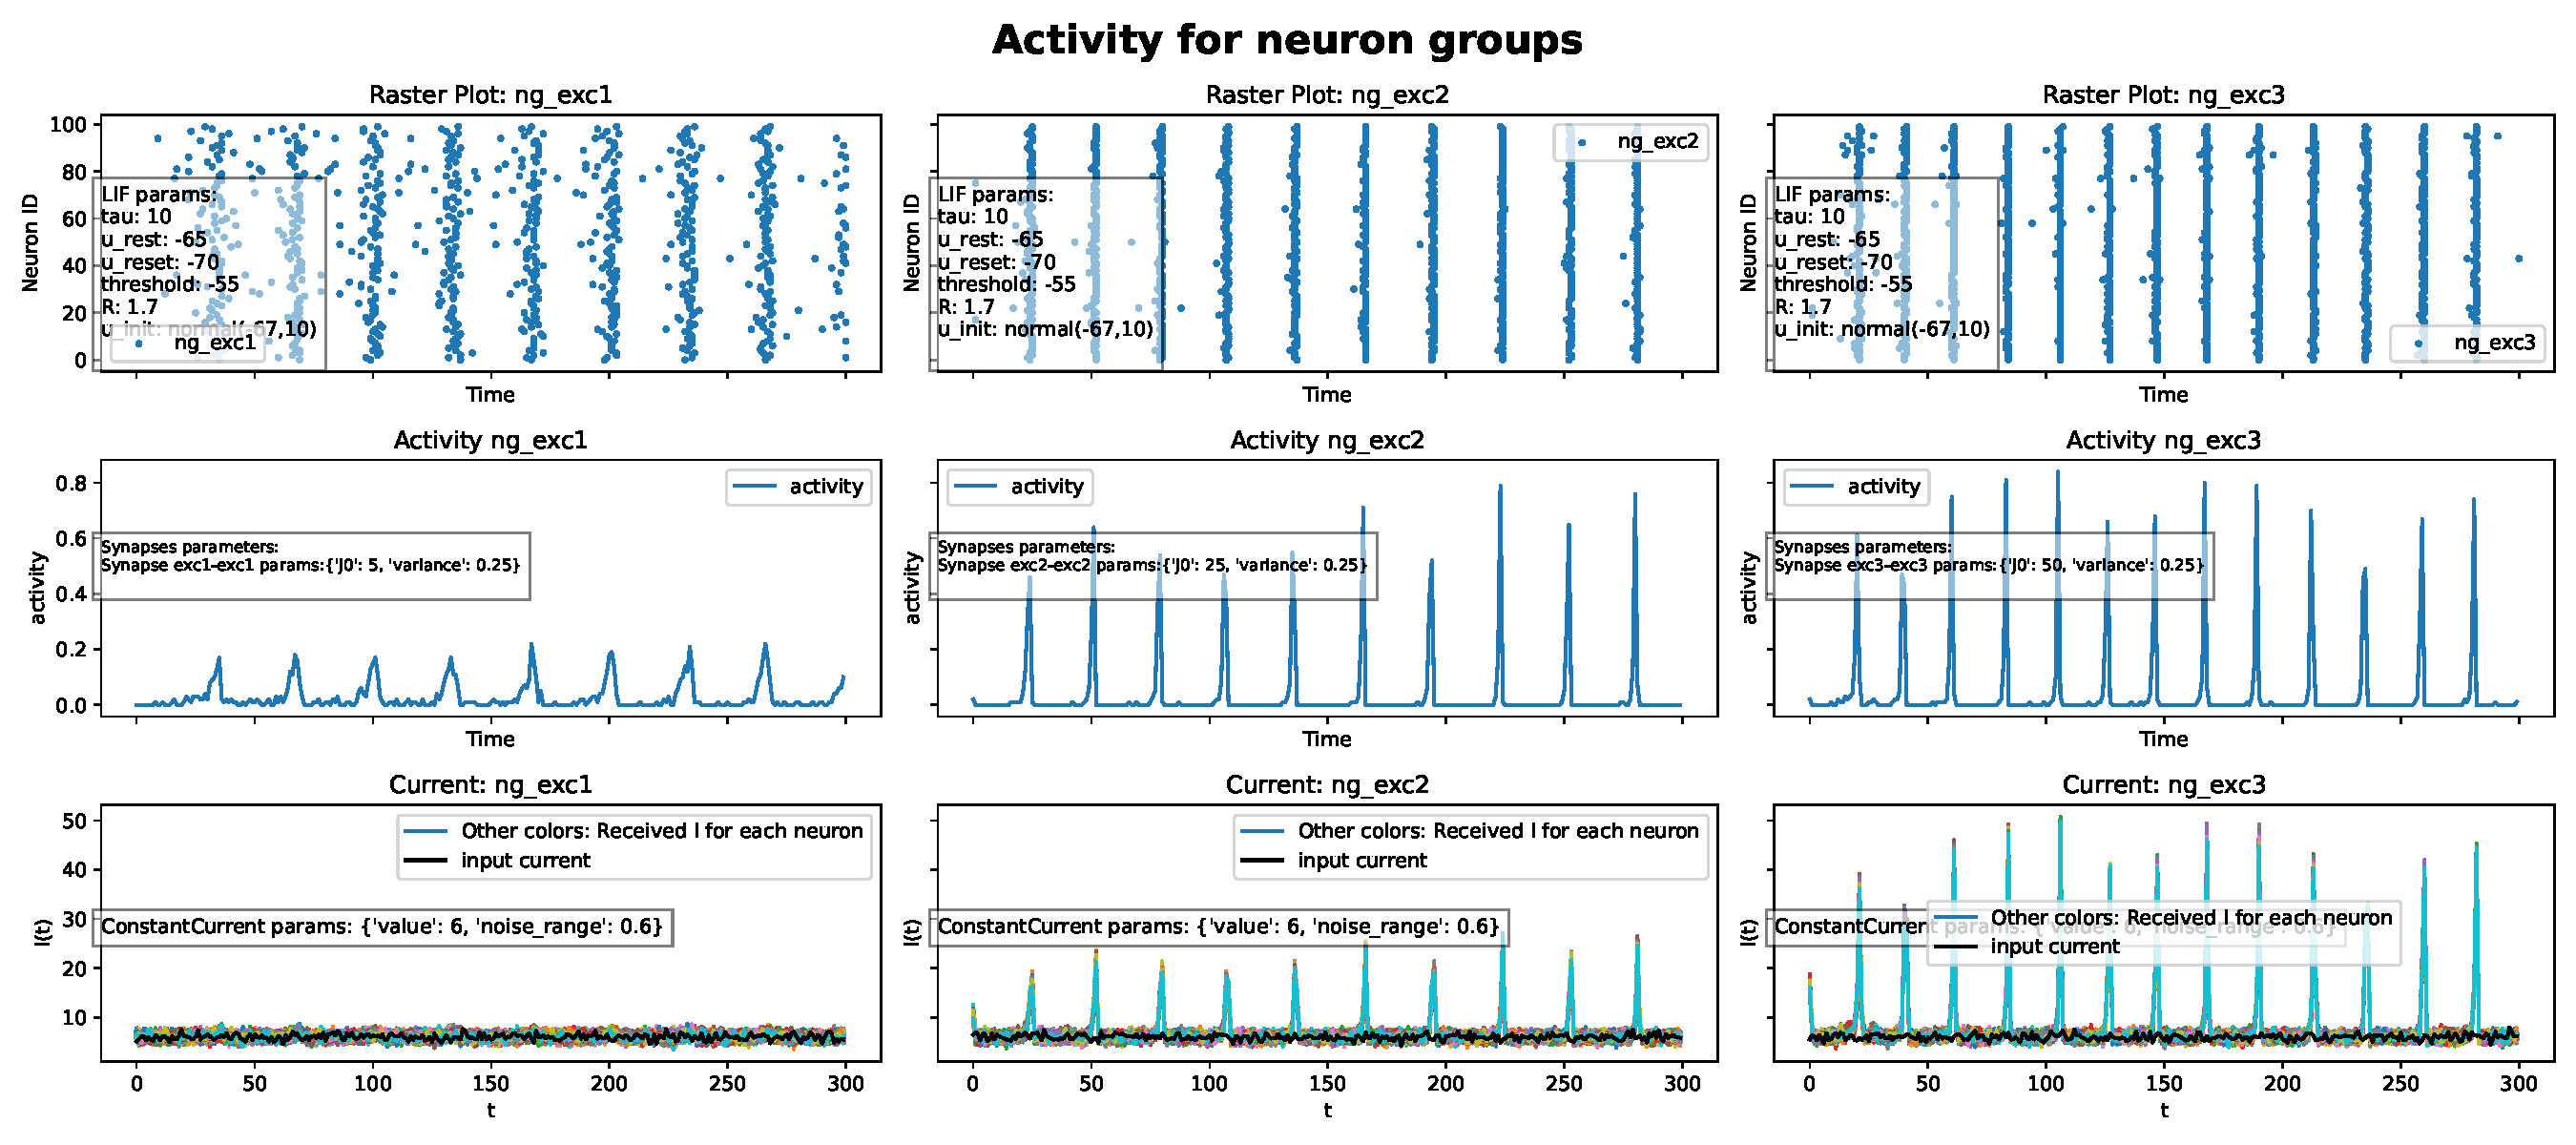
\includegraphics[width=0.9\textwidth]{plots/part2-one-ng-full-synapse-diff-j.pdf} 
                    \caption{رفتار یک جمعیت نورونی با مقادیر $j_0$ مختلف و جریان ثابت نویز دار}
                    \label{fig:part2-one-ng-full-synapse-diff-j}
                \end{figure}

                حال به جمعیت نورونی مان، یک جریان تصادفی میدهیم تا رفتار شبیه به نورون واقعی را بیشتر بررسی کنیم. مجددا در شکل
                \ref{fig:part2-one-ng-full-synapse-diff-j-rand-curr}
                مشاهده میکنیم که تصادفی بودن جریان، منجر به پراکندگی زمان ضربه زدن نورون ها می شود و به طور کلی فعالیت آن ها را کاهش داده است، اما با زیاد کردن وزن های سیناپسی، این نوسانات کمتر شده به طور که در نمودار سمت راست، میتوانیم زمان ضربه زدن نورون ها را در ستون هایی دسته بندی کنیم.
                \begin{figure}[!ht]
                    \centering
                    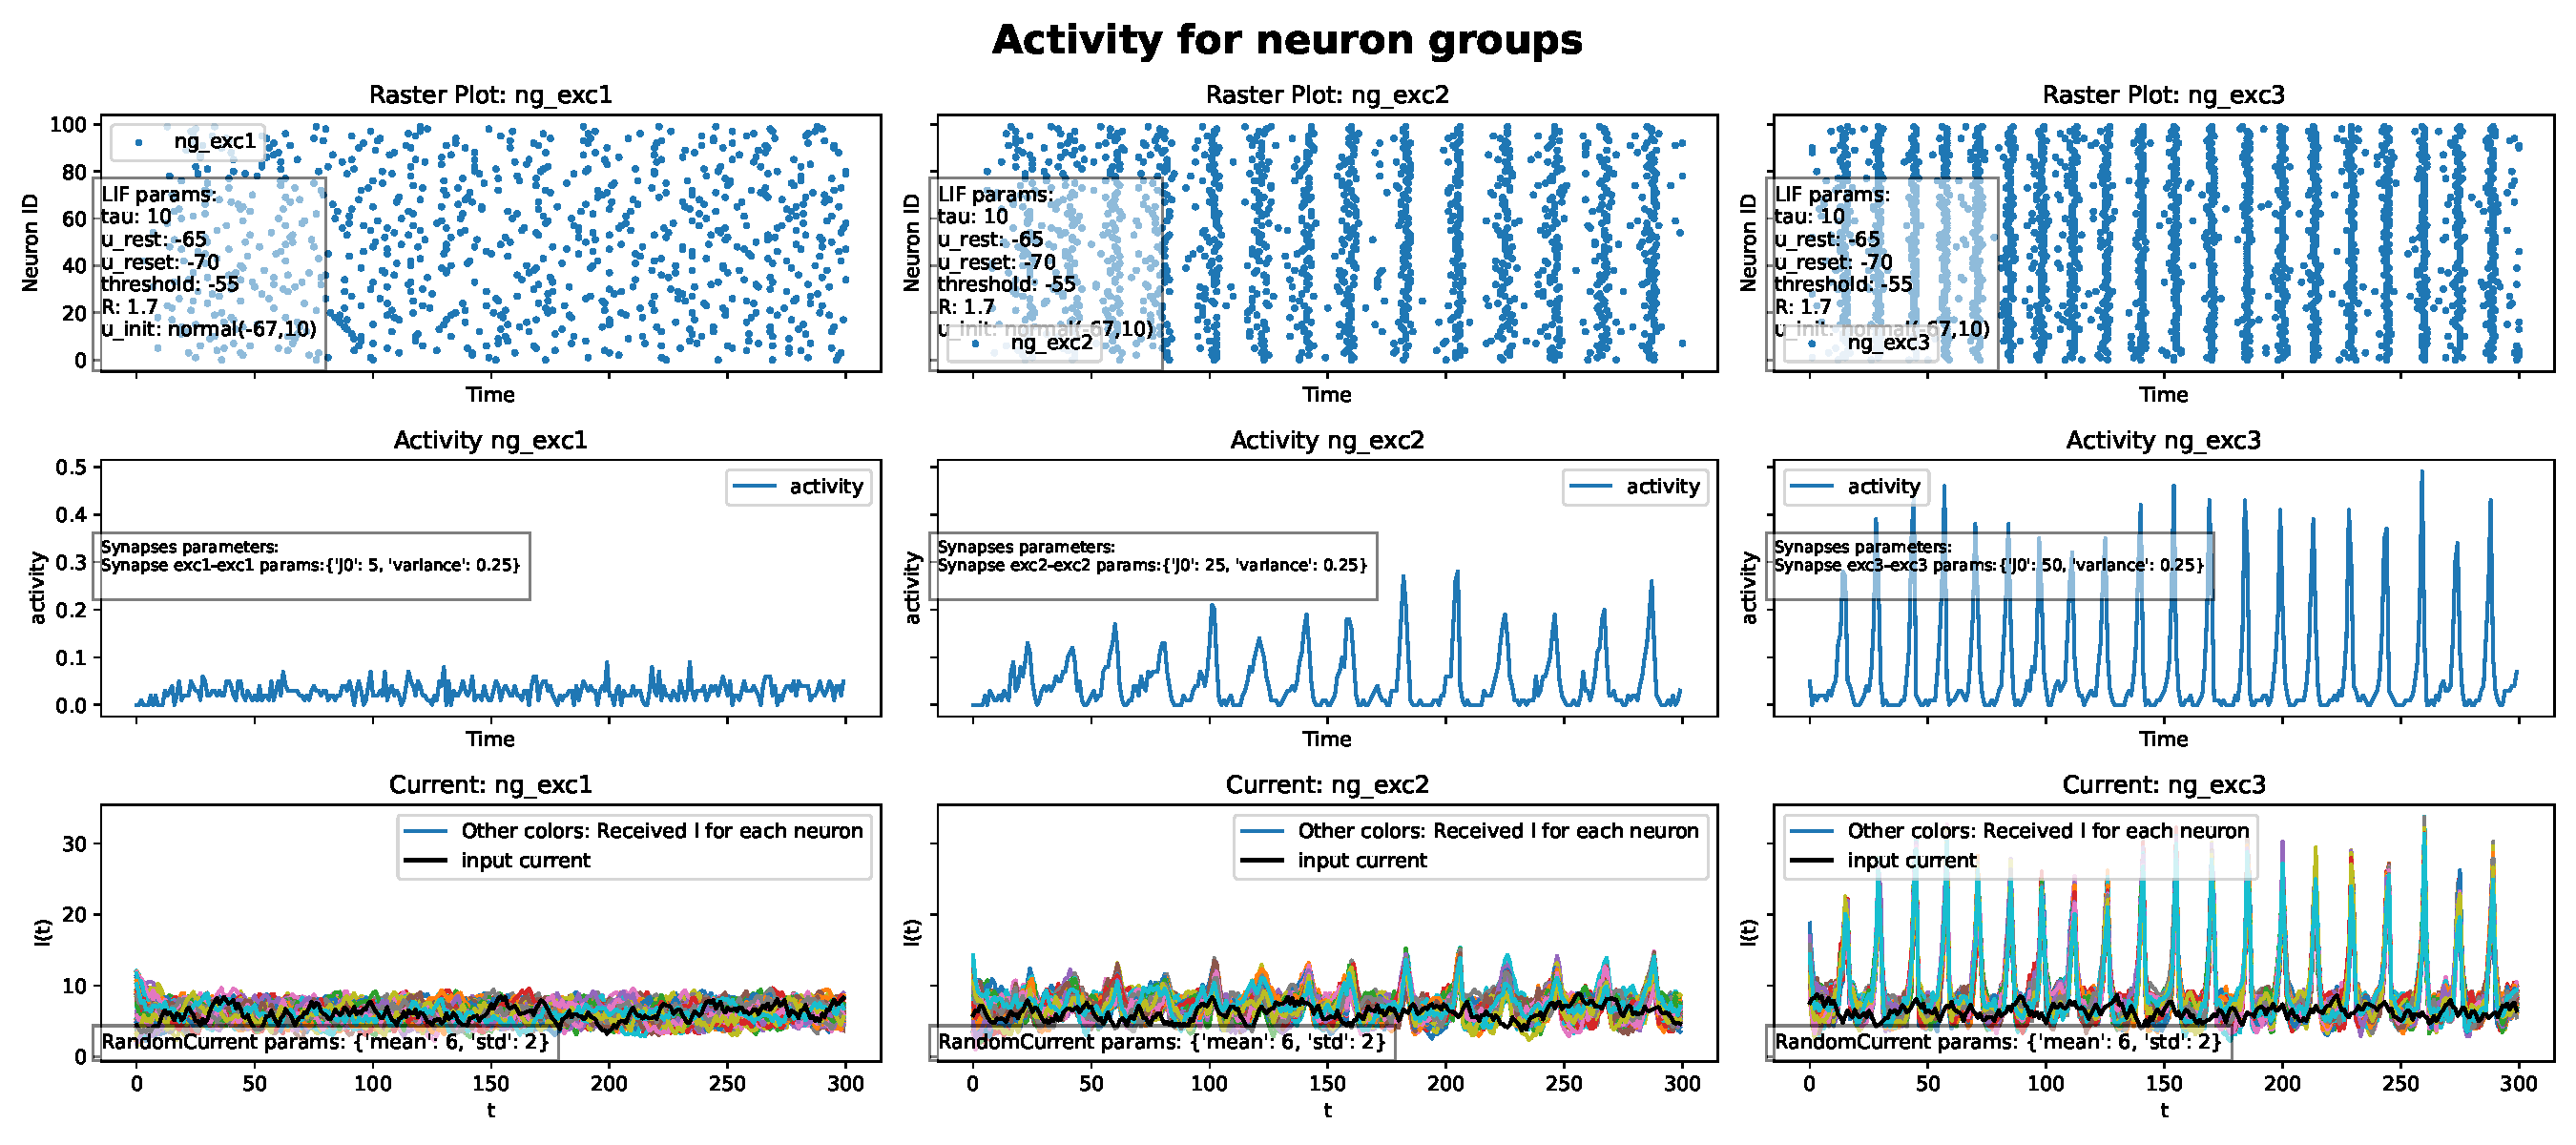
\includegraphics[width=0.9\textwidth]{plots/part2-one-ng-full-synapse-diff-j-rand-curr.pdf} 
                    \caption{رفتار یک جمعیت نورونی با مقادیر $j_0$ مختلف و جریان تصادفی}
                    \label{fig:part2-one-ng-full-synapse-diff-j-rand-curr}
                \end{figure}

            \paragraph*{پارامتر واریانس}
                حال رفتار جمعیت را به ازای مقادیر مختلف واریانس تحلیل میکنیم. برای این قسمت نیز از همان مدل نورونی بالا استفاده میکنیم. از آنجا که الگوی ارتباطی مان کامل است، انتظار داریم که تغییر معقول واریانس تفاوت زیادی در رفتار کلی نورون ها ایجاد نکند، چرا که هر نورون با تمام نورون های دیگر ارتباط دارد و از این رو برآیند جریان سناپسی وارد شده به نورون ها نزدیک به هم می باشد. شکل 
                \ref{fig:part2-one-ng-full-synapse-diff-variance}
                بیانگر همین موضوع است. هر چند تغییرات کوچکی میتواند رخ دهد. مثلا در نمودار سمت راست که واریانس برابر با خود میانگین دارد
                (گفتیم که عددی که به عنوان واریانس به مدل ورودی داده می شود در میانگین ضرب شده و سپس تشکیل واریانس اصلی توزیع را می دهد)،
                میزان فعالیت کلی نورون ها کمی از دو مدل دیگر بیشتر است.
                \begin{figure}[!ht]
                    \centering
                    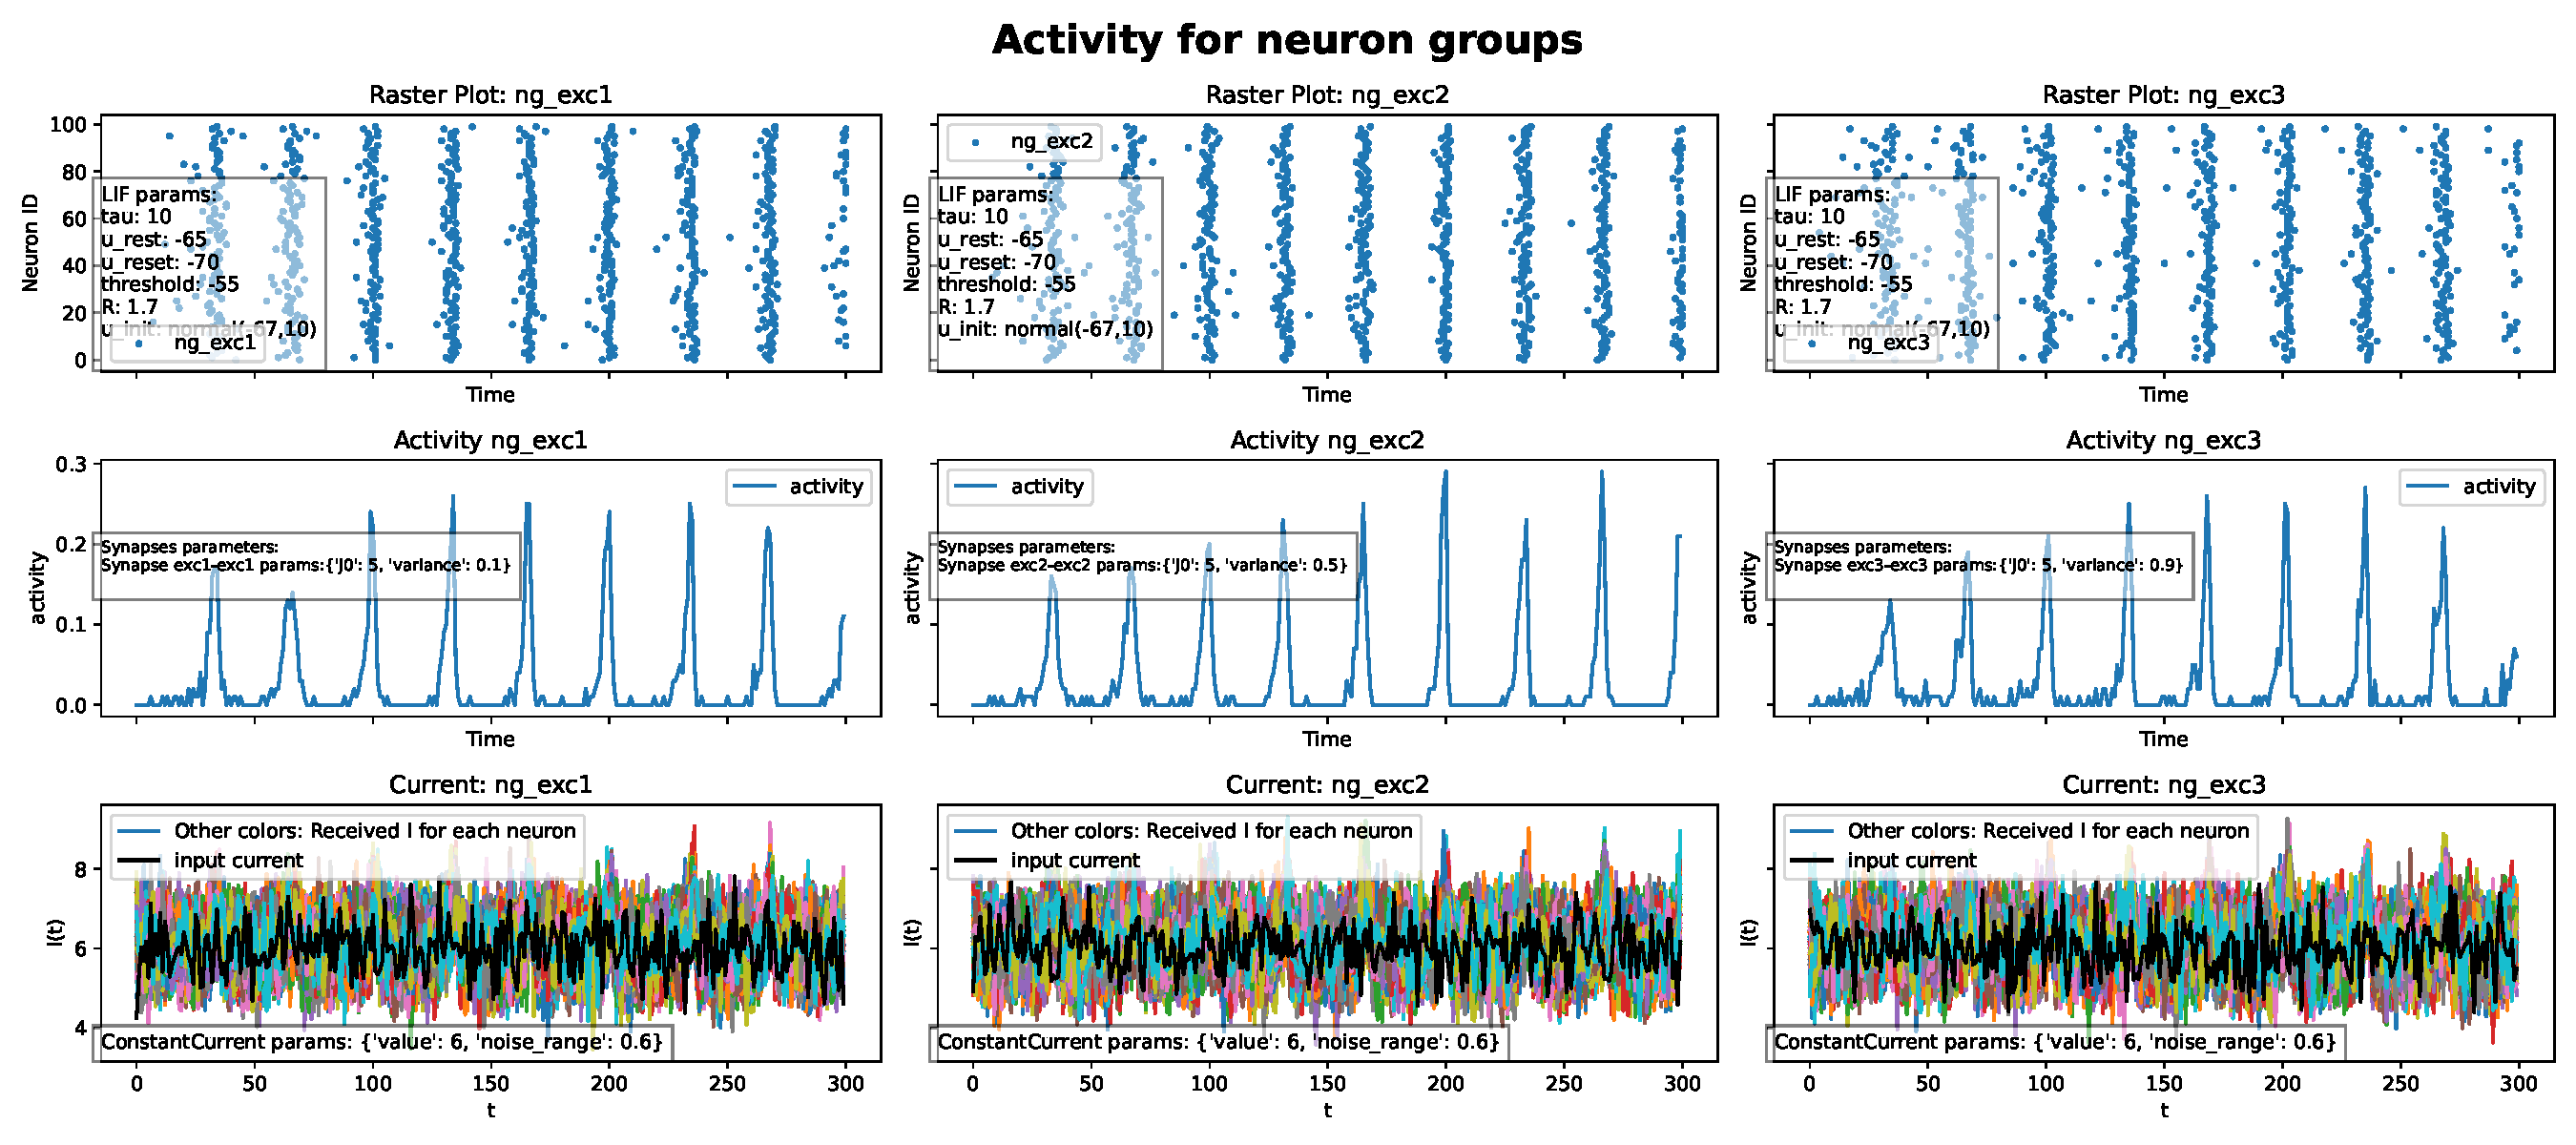
\includegraphics[width=0.9\textwidth]{plots/part2-one-ng-full-synapse-diff-variance.pdf} 
                    \caption{رفتار یک جمعیت نورونی با واریانس مختلف و جریان ثابت نویزدار}
                    \label{fig:part2-one-ng-full-synapse-diff-variance}
                \end{figure}

                حال رفتار را با یک جریان تصادفی آزمایش می کنیم. در جریان تصادفی نیز مطابق شکل
                \ref{fig:part2-one-ng-full-synapse-diff-variance-rand-curr}
                دریافت می شود که تغییر واریانس تاثیر چندانی بر روی رفتار جمعیت ندارد. به طور کلی میتوان این نتیجه را گرفت که در الگوی ارتباط کامل با جریان غیر ثابت، به دلیل اینکه همه نورون ها با یکدیگر در ارتباط هستند، افزودن واریانس به وزن ها نمیتواند روی جریان تصادفی تاثیر بگذارد.

                \begin{figure}[!ht]
                    \centering
                    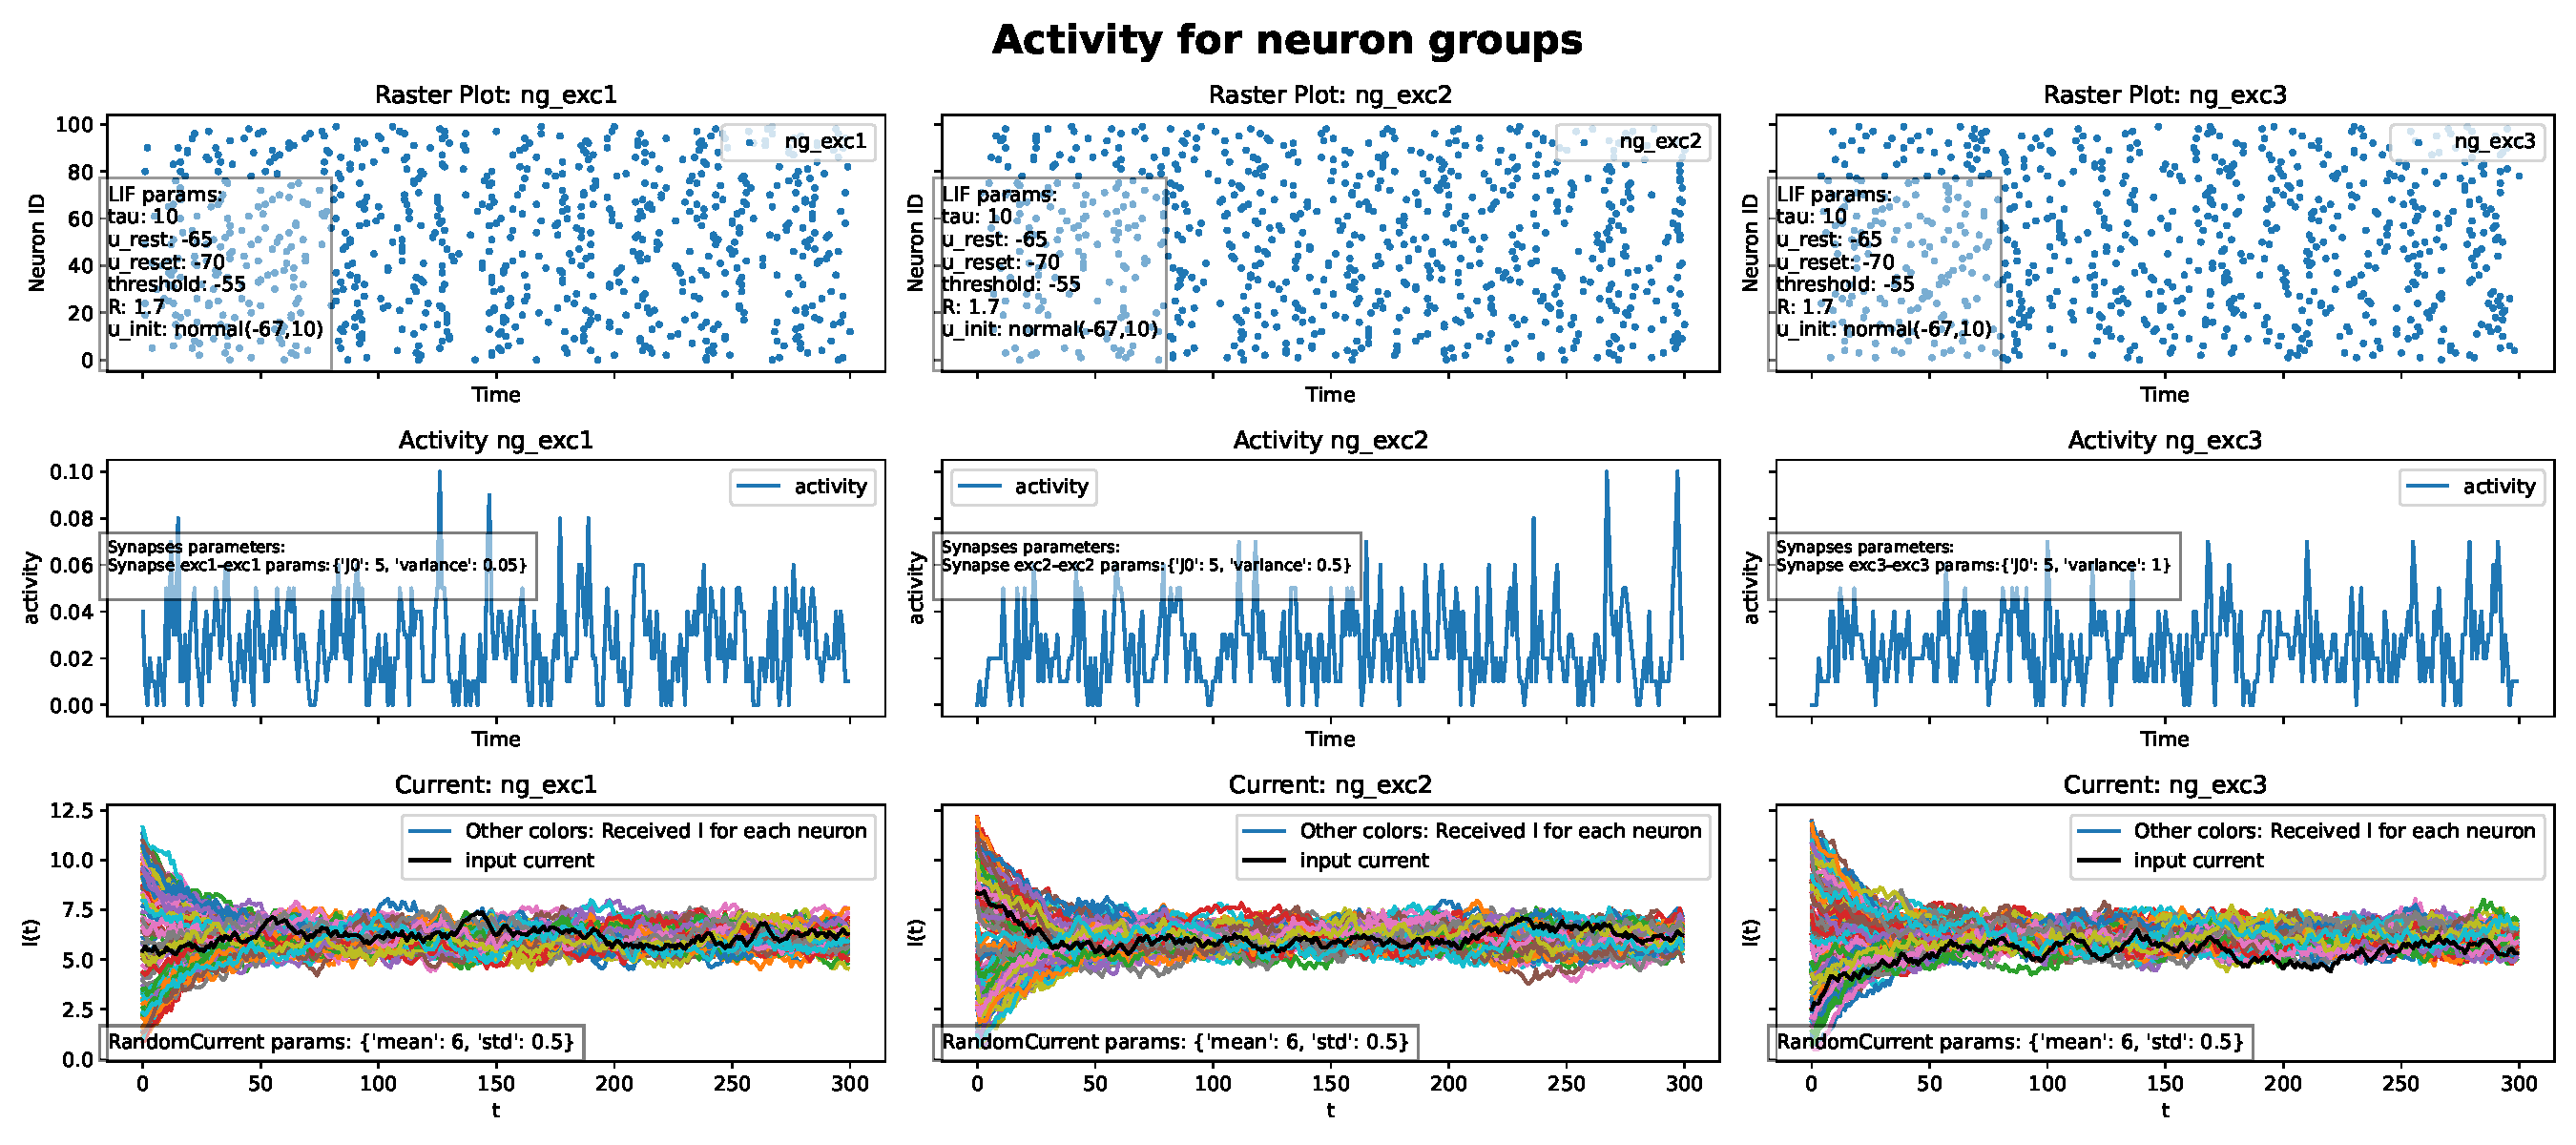
\includegraphics[width=0.9\textwidth]{plots/part2-one-ng-full-synapse-diff-variance-rand-curr.pdf} 
                    \caption{رفتار یک جمعیت نورونی با واریانس مختلف و جریان تصادفی}
                    \label{fig:part2-one-ng-full-synapse-diff-variance-rand-curr}
                \end{figure}

            \paragraph*{اندازه جمعیت}
                خالی از لطف نیست که تاثیر اندازه جمعیت را روی رفتار آن بررسی میکنیم. برای اینکار سه جمعیت نورونی به اندازه های ۵۰، ۱۰۰ و ۲۵۰ را بررسی میکنیم تا ببینیم اندازه چه تاثیری روی رفتار جمعیت دارد. طبق شکل
                \ref{fig:part2-one-ng-full-synapse-diff-size}
                مشاهده می کنیم که اگر مدل نورون ها و جریان را یکی بگیریم، برای جمعیت با اندازه های متفاوت، فعالیت نورونی تغییری نکرده و مستقل از اندازه جمعیت است.
                \begin{figure}[!ht]
                    \centering
                    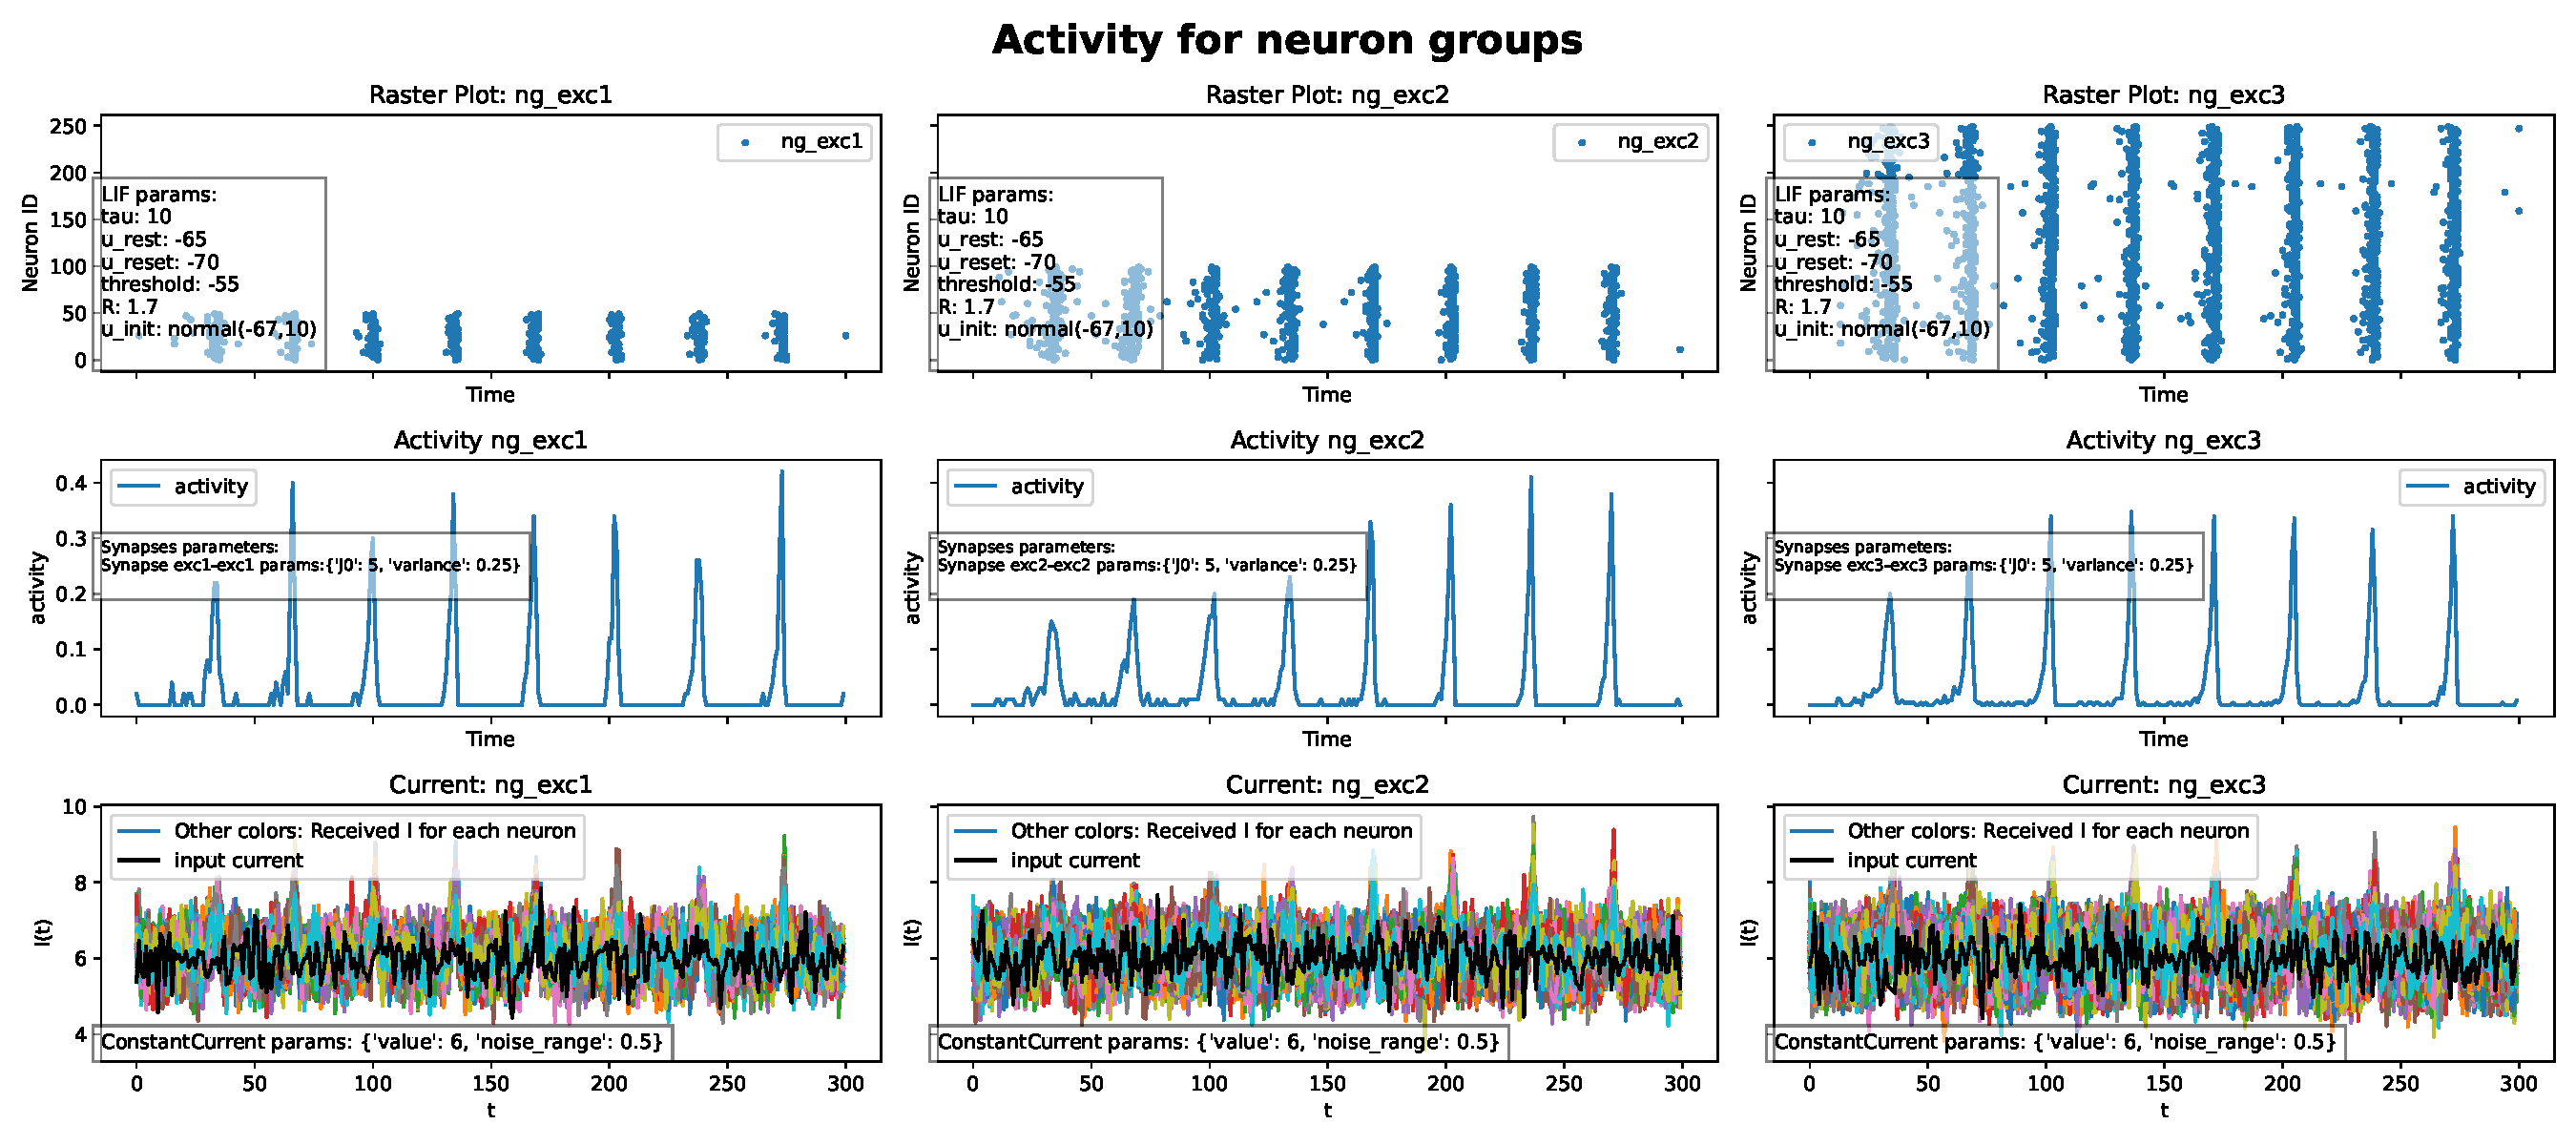
\includegraphics[width=0.9\textwidth]{plots/part2-one-ng-full-synapse-diff-size.pdf} 
                    \caption{رفتار یک جمعیت نورونی با جمعیت مختلف و جریان تصادفی}
                    \label{fig:part2-one-ng-full-synapse-diff-size}
                \end{figure}
            \paragraph*{مدل های نورونی}
                در نهایت نیز به سراغ بررسی تاثیر انتخاب مدل نورونی روی رفتار جمعیت میرویم. همانطور که از شکل
                \ref{fig:part2-one-ng-full-synapse-diff-neuron-model}
                پیداست، رفتار مدل نورونی 
                $LIF$ و
                $ELIF$ 
                شبیه یکدیگر است در حالی که در مدل 
                $AELIF$ 
                با گذر زمان، فعالیت نورونی کاهش یافته و به مقدار کمتری همگرا می شود. هر چند من خیلی هنگام پیاده سازی روی قسمت های ۲ مدل دیگر مانور ندادم و ممکن است دقیق نباشند.
                \begin{figure}[!ht]
                    \centering
                    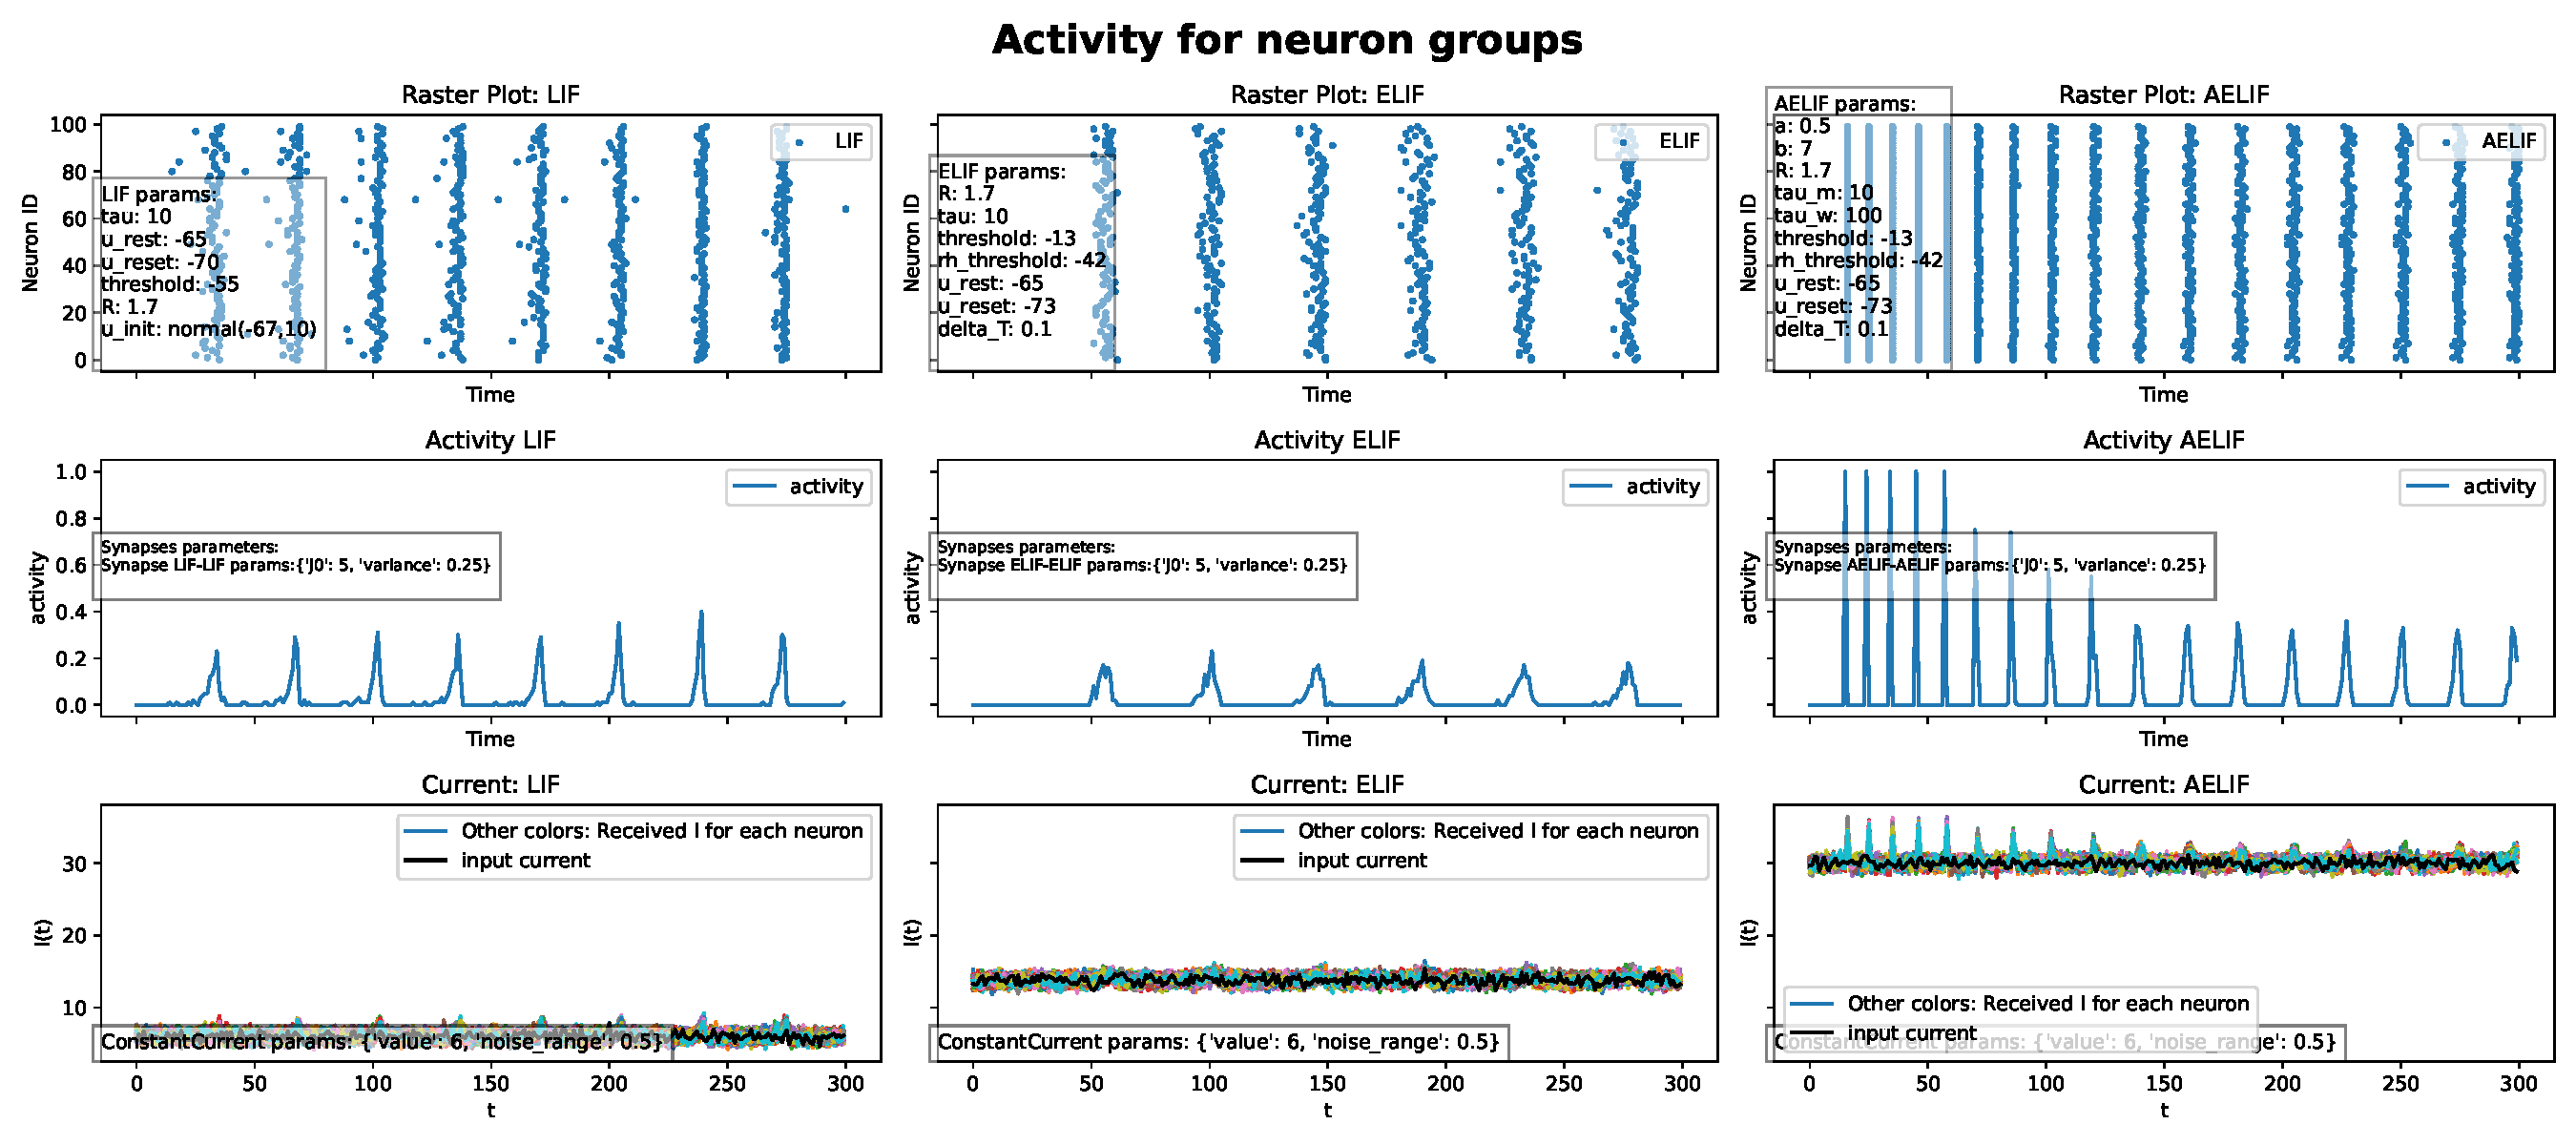
\includegraphics[width=0.9\textwidth]{plots/part2-one-ng-full-synapse-diff-neuron-model.pdf} 
                    \caption{رفتار یک جمعیت نورونی با مدل های نورونی مختلف و جریان تصادفی}
                    \label{fig:part2-one-ng-full-synapse-diff-neuron-model}
                \end{figure}
        \subsubsection{بررسی رفتار دو جمعیت}
            \paragraph*{پارامتر $j_0$}
            حال به بررسی رفتار دو جمعیت که بین آن ها سیناپس قرار دارد می پردازیم. در این بخش   تاثیر دو جمعیت روی یکدیگر را بررسی میکنیم. اولین حالتی که مورد بررسی قرار می دهیم، حالتی است که دو حمعیت تحریکی هستند و فقط به یکدیگر سیناپس دارند و سیناپس داخلی بین نورون های آن ها وجود ندارد.
            در این حالت با نتایجی که تا الآن بدست آورده ایم انتظار داریم که فعالیت دو جمعیت شبیه یک دیگر باشند که شکل
            \ref{fig:part2-two-ng-full-synapse-noise-curr}
            نیز این موضوع را تایید میکند. جریان تصادفی نیز رفتار مشابهی از خود نشان می دهد. 
            (شکل \ref{fig:part2-two-ng-full-synapse-rand-curr})
            \begin{figure}[!ht]
                \centering
                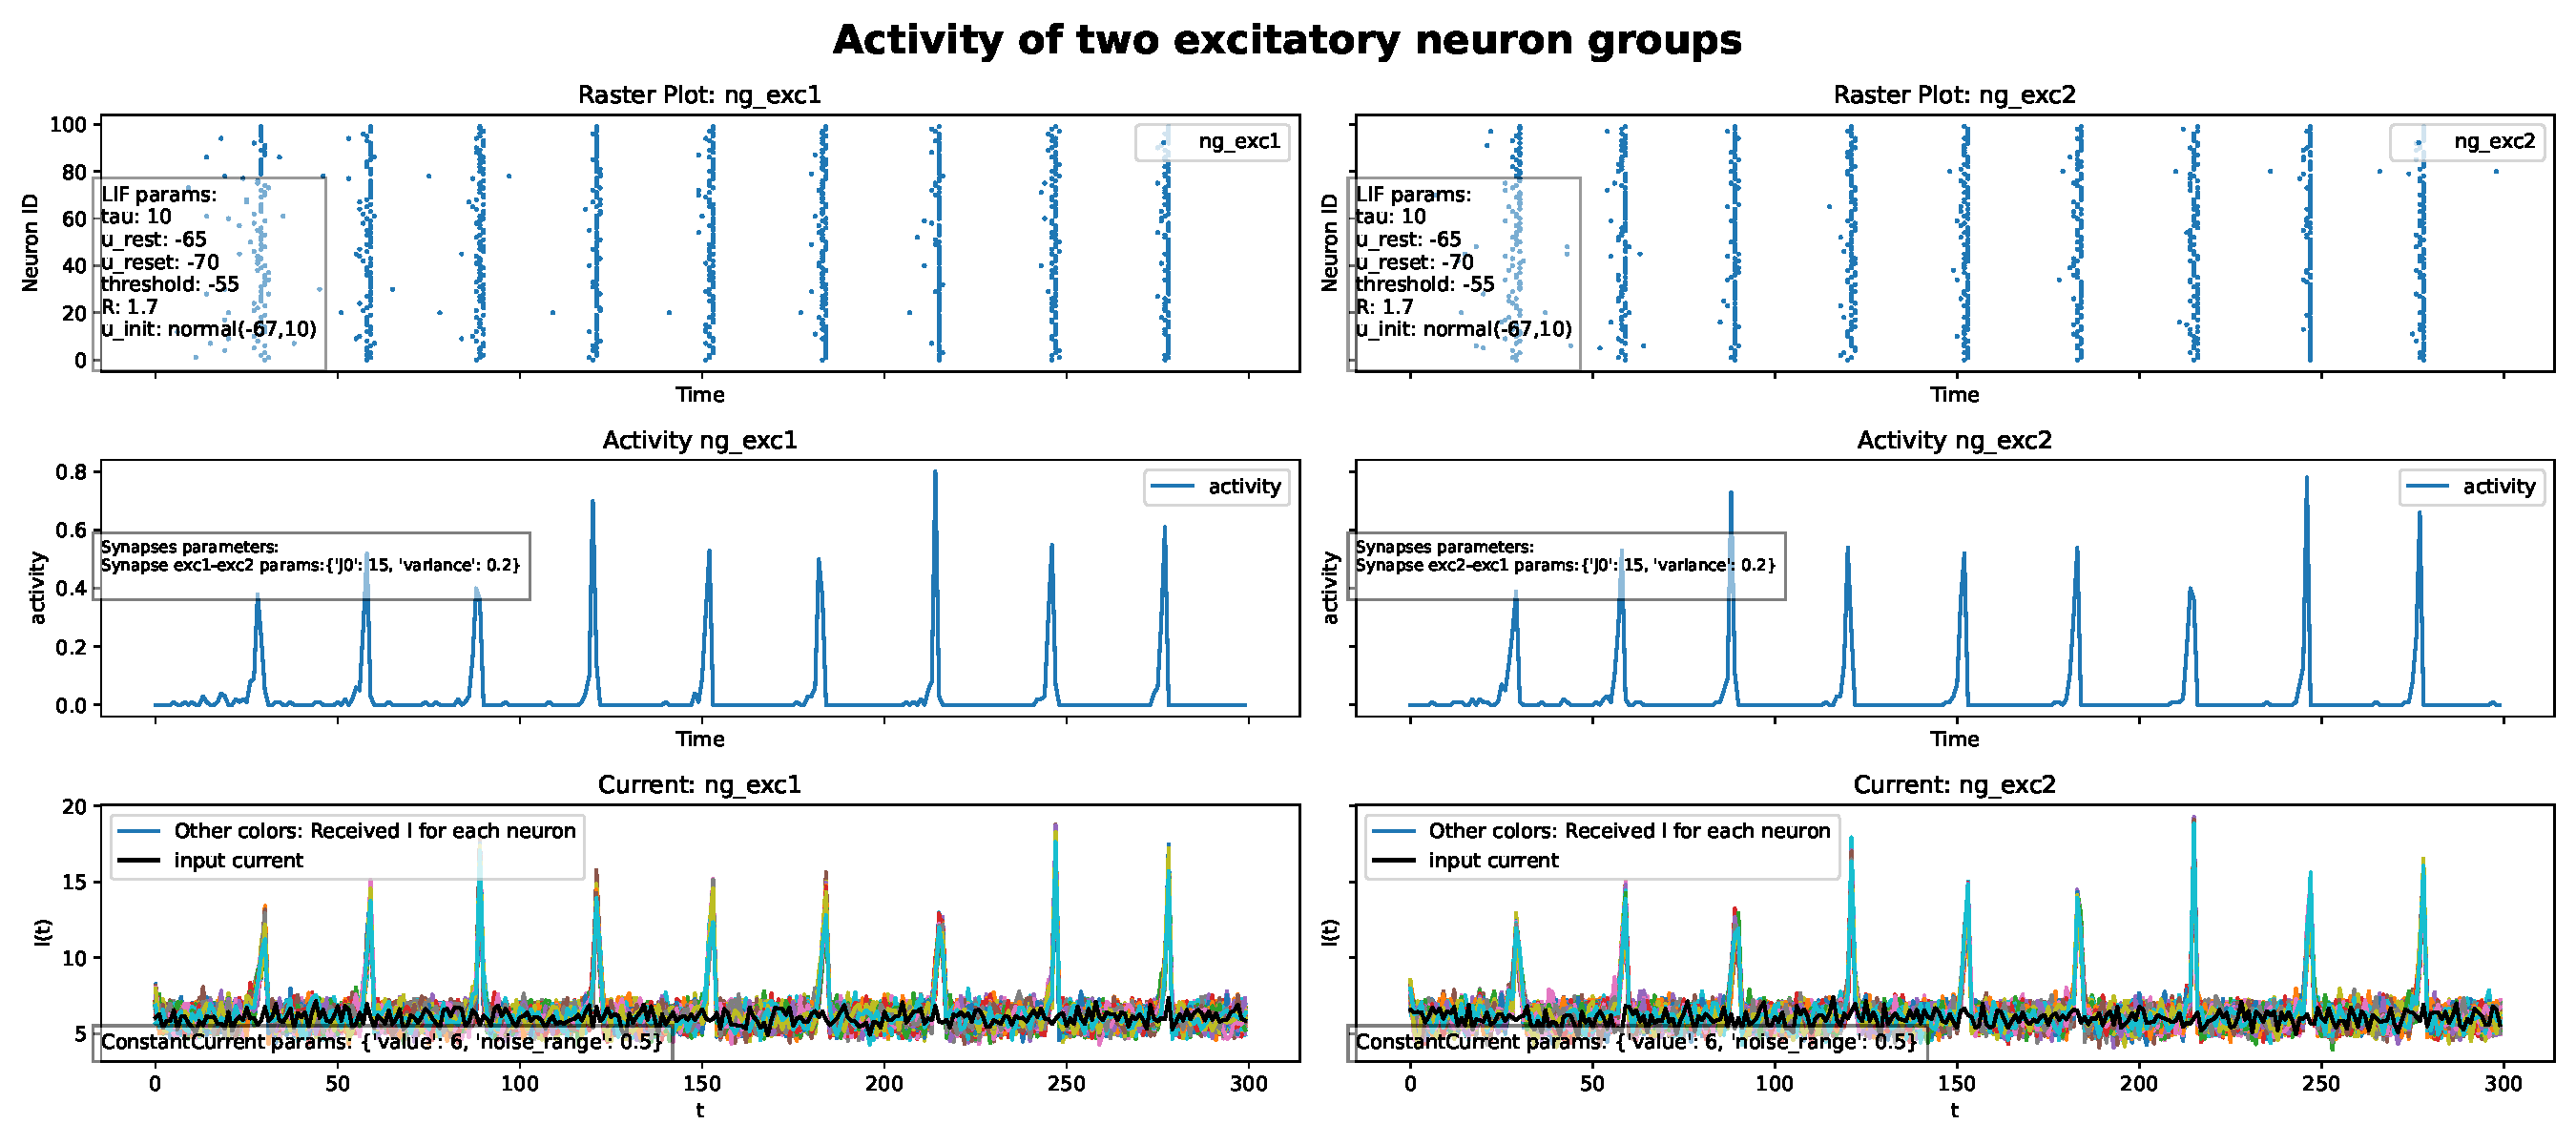
\includegraphics[width=0.9\textwidth]{plots/part2-two-ng-full-synapse-noise-curr.pdf} 
                \caption{رفتار دو جمعیت نورونی با دو سیناپس و جریان ثابت نویزی}
                \label{fig:part2-two-ng-full-synapse-noise-curr}
            \end{figure}
            \begin{figure}[!ht]
                \centering
                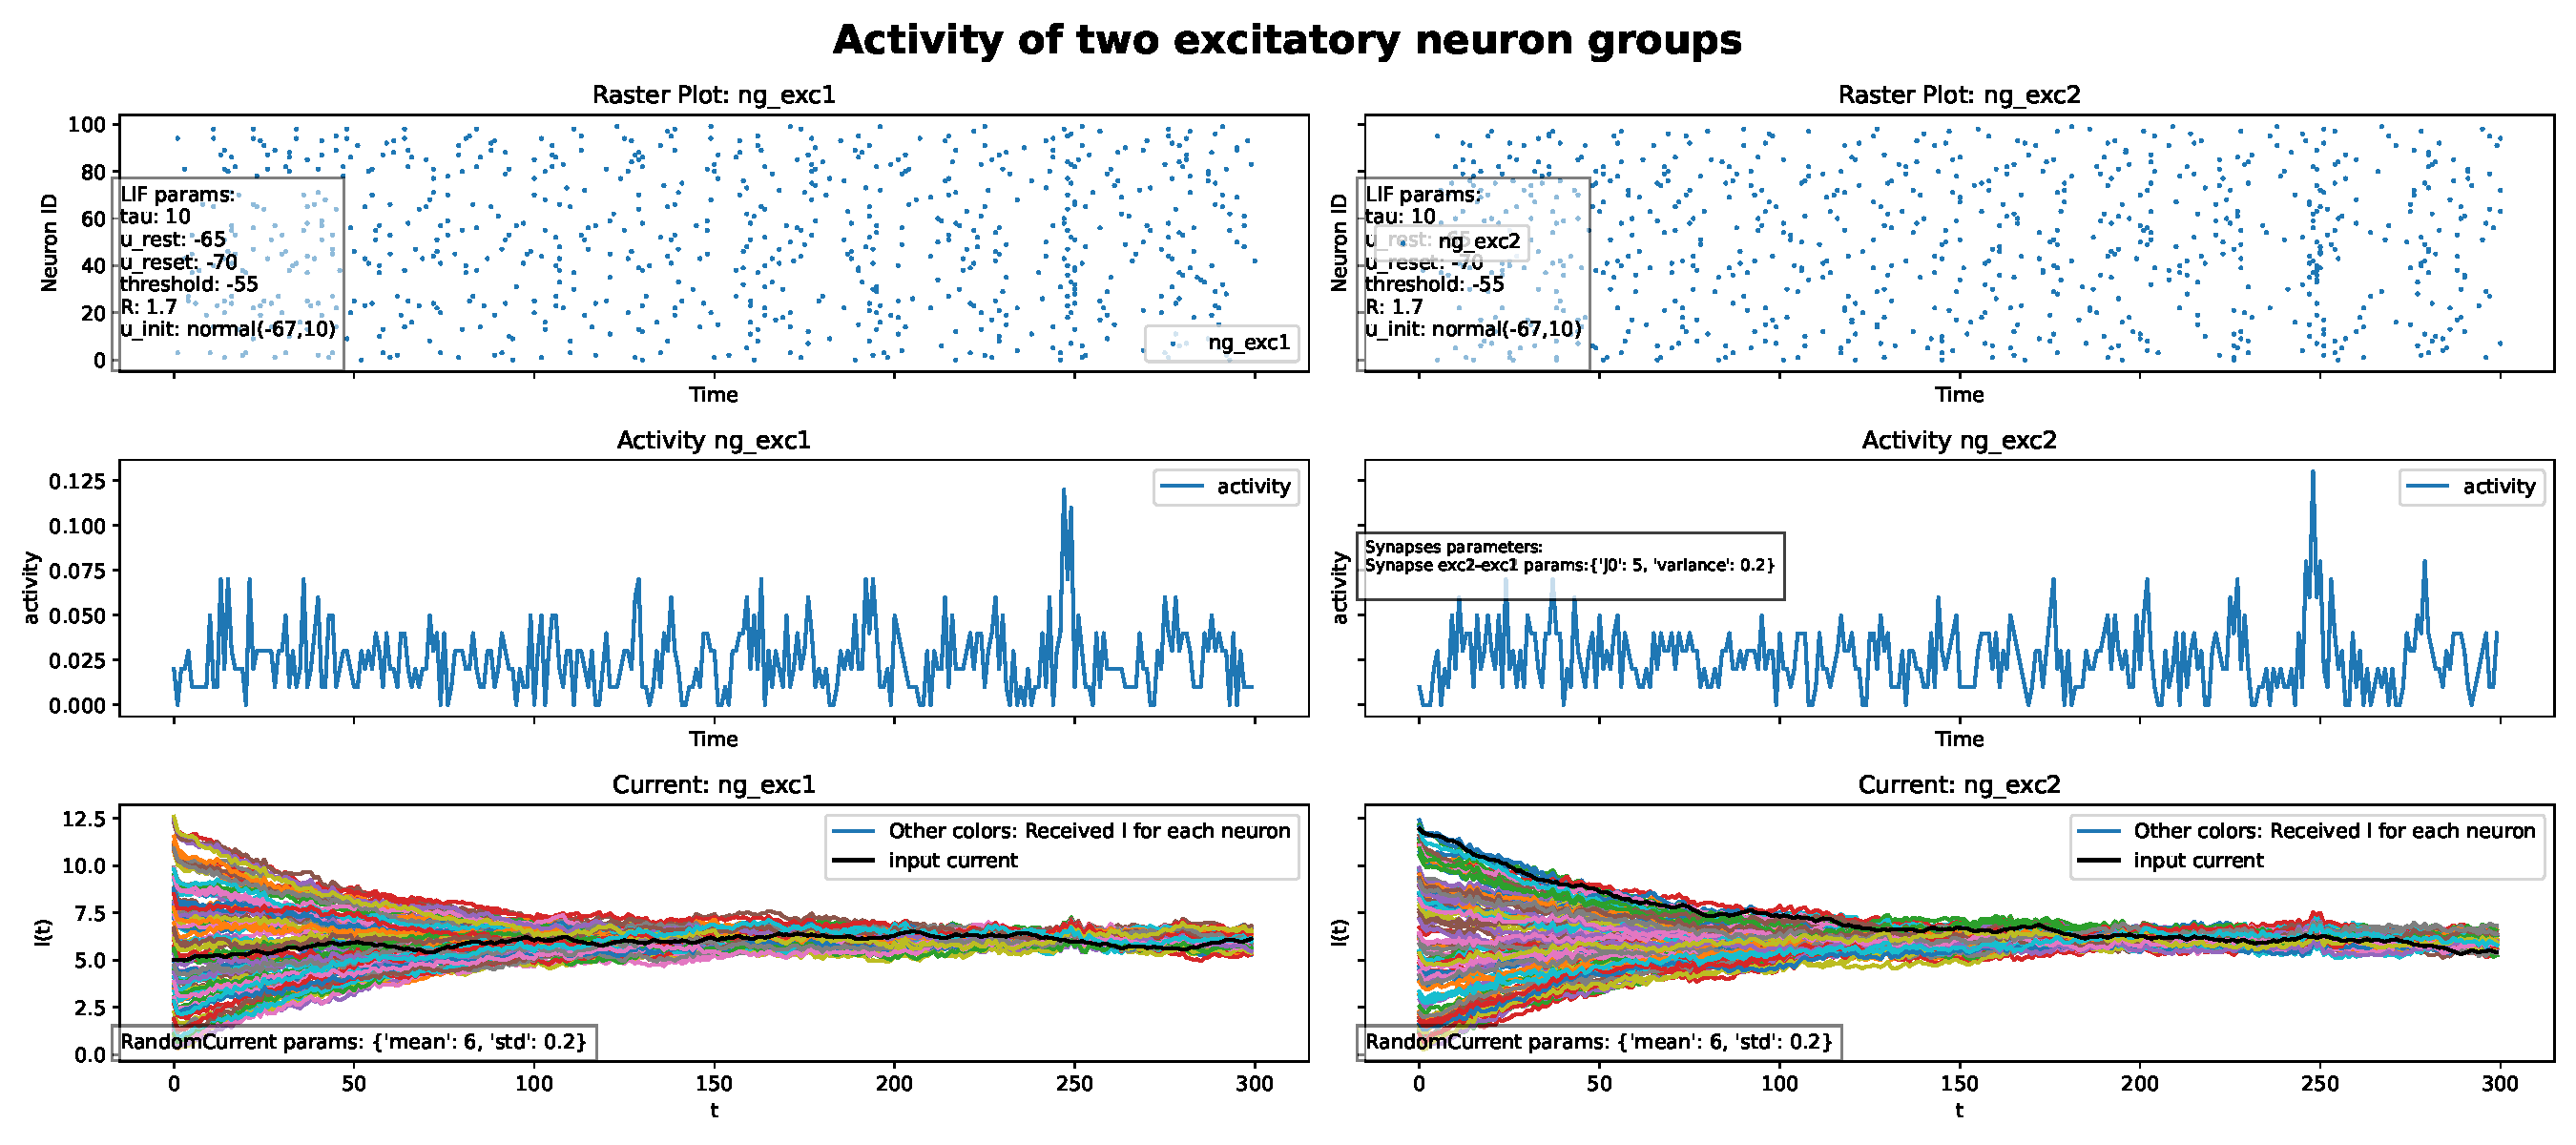
\includegraphics[width=0.9\textwidth]{plots/part2-two-ng-full-synapse-rand-curr.pdf} 
                \caption{رفتار دو جمعیت نورونی با دو سیناپس و جریان تصادفی}
                \label{fig:part2-two-ng-full-synapse-rand-curr}
            \end{figure}

            رفتار جالب دیگری که جریان تصادفی دارد، این است که در ابتدا پراکندگی زمان ضربه زدن نورون ها بسیار زیاد است و الگوی خاصی ندارد، و همچنین فعالیت نورونی کم است، اما همانطور که از نمودار پیداست، این پراکندگی رفته رفته کمتر شده و فعالیت نورونی نیز بیشتر می شود. این اتفاق تحت تاثیر این موضوع است که به دلیل وجود سنیاپس بین دو جمعیت که به صورت رفت و برگشتی است، به گونه ای عمل کرده که هر نورون از تمام نورون های جمعیت دیگر جریان دریافت میکند و درنتیجه جریان دریافتی به نورون زیاد می شود و این جریان زیاد باعث می شود تا پس از مدتی زمان ضربه زدن نورون ها به یکدیگر نزدیک شود.

            حال اگر مقدار 
            $j_0$ 
            را در هر ۲ سیناپس کاهش دهیم چه اتفاقی می افتد؟ شکل 
            \ref{fig:part2-two-ng-full-synapse-low-j-rand-curr}
            به این سوال پاسخ می دهد و بیان می کند که کاهش مقدار 
            $j_0$ 
            باعث می شود تا جریان سیناپسی نتواند آنقدر زیاد شود که در زمان قبلی پراکندگی فعالیت نورون ها را کمتر کند و فعالیت جمعیت به صورت یک نمودار تصادفی با مقدار کم باقی می ماند.(این نکته در بخش های بعدی به کارمان می آید.)
            \begin{figure}[!ht]
                \centering
                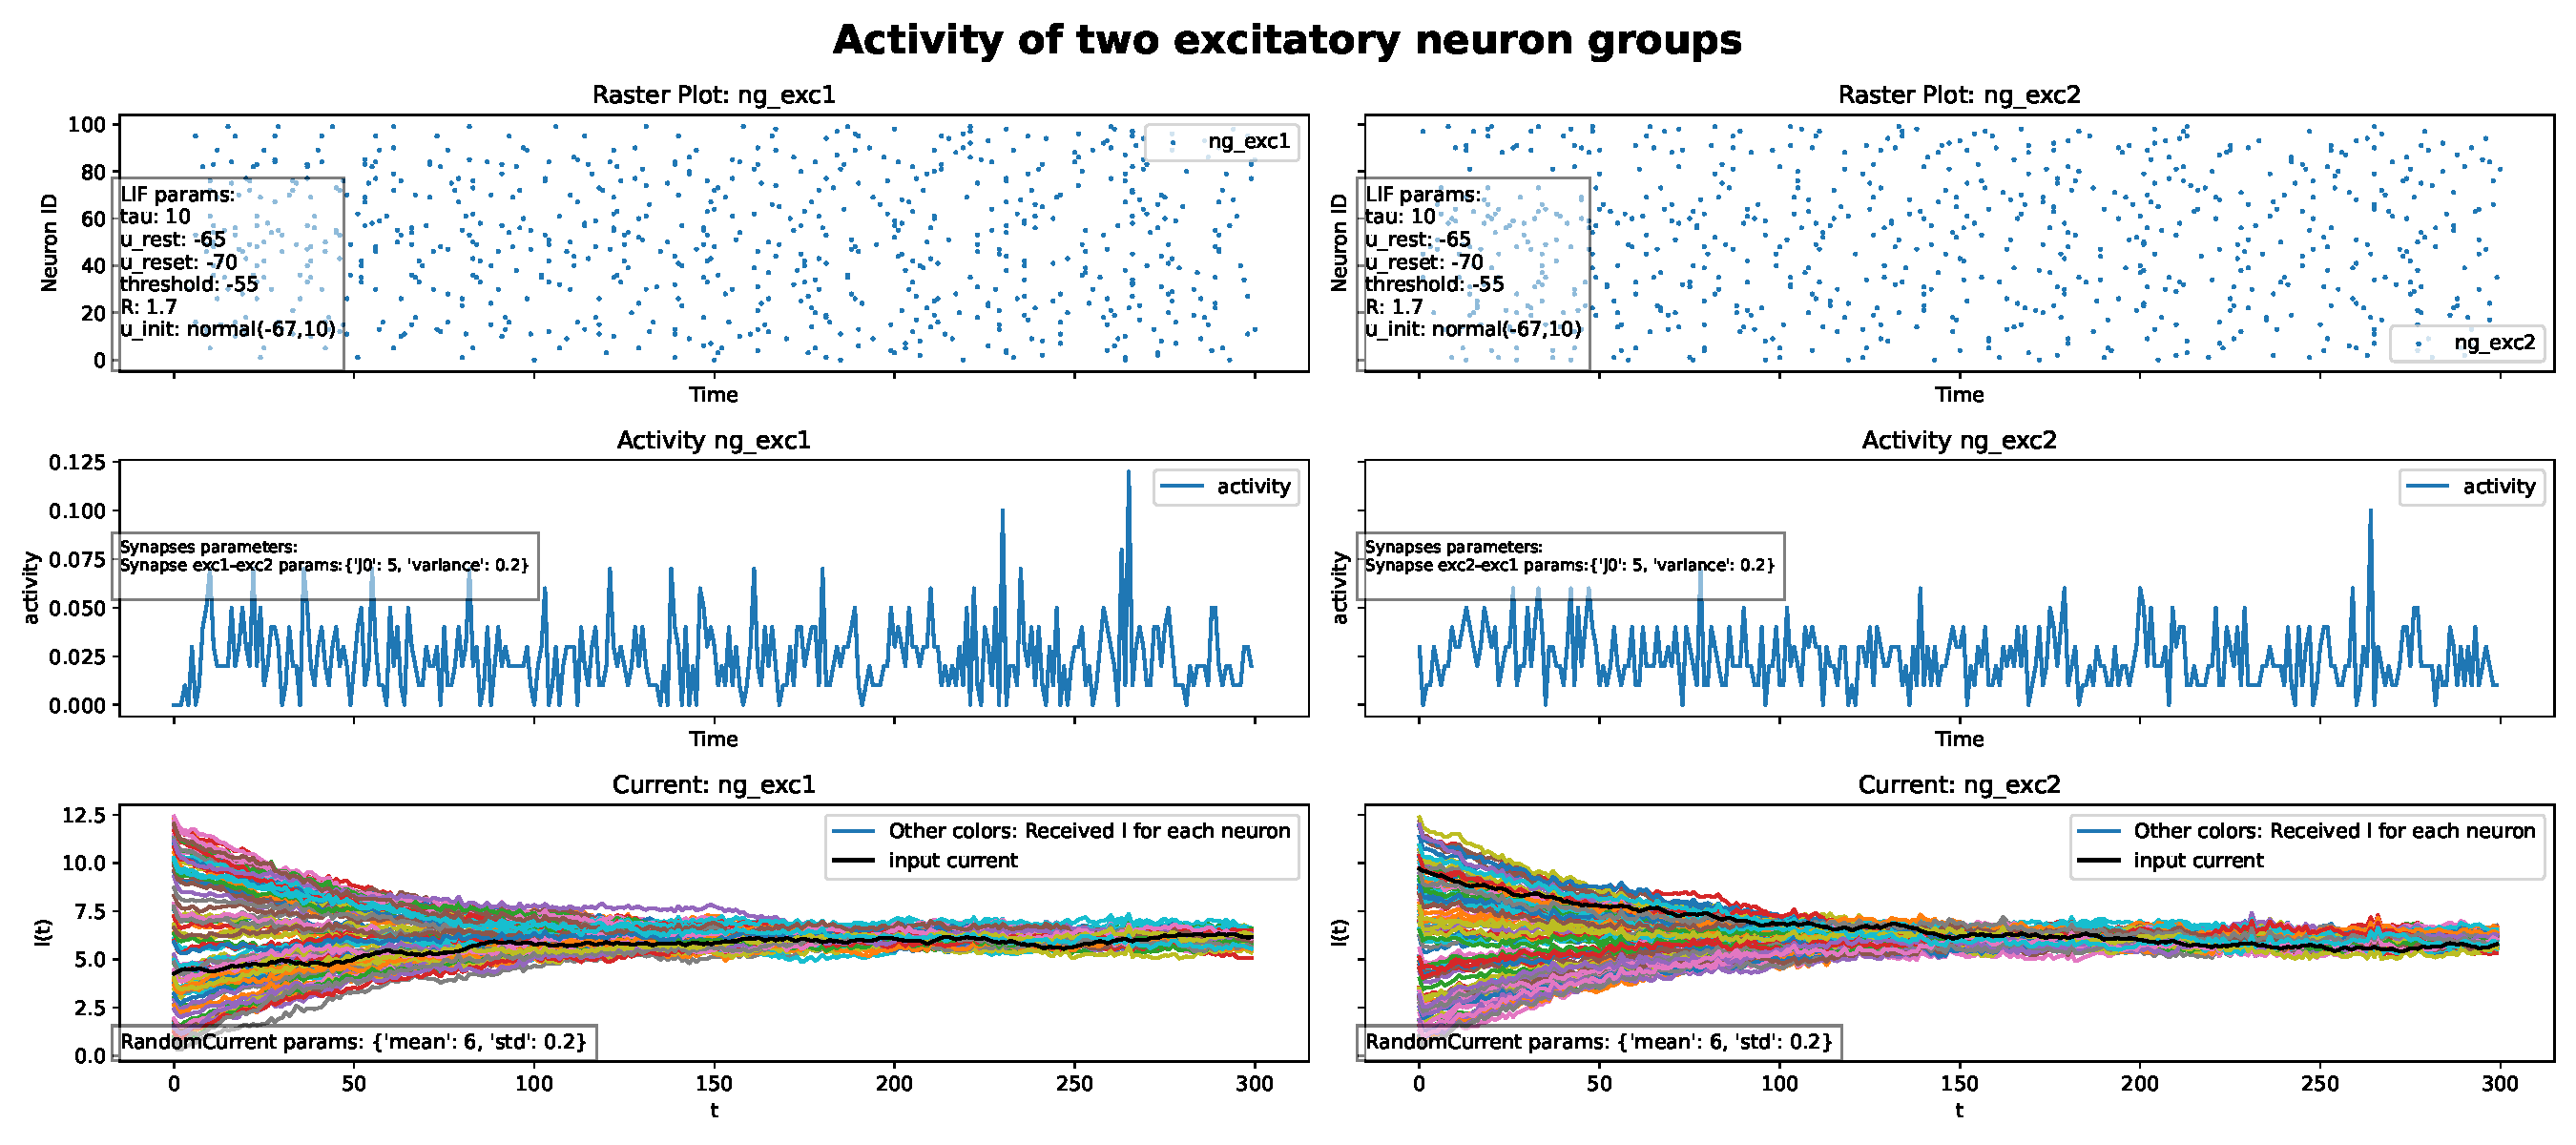
\includegraphics[width=0.9\textwidth]{plots/part2-two-ng-full-synapse-low-j-rand-curr.pdf} 
                \caption{رفتار دو جمعیت نورونی با دو سیناپس و جریان تصادفی و $j_0$ کم}
                \label{fig:part2-two-ng-full-synapse-low-j-rand-curr}
            \end{figure}

            حال مقدار وزن های سیناپس بین جمعیت ۱ به جمعیت ۲ را افزایش میدهیم تا ببینیم با 
            $j_0$
            متفاوت رفتار آن ها چه تغییری میکند. طبق شکل 
            \ref{fig:part2-two-ng-full-synapse-diff-j-rand-curr}
            مشاهده میکنیم که فعالیت هر دو جمعیت بیشتر شده ولی جمعیت ۲ در کل فعالیت بیشتری دارد. مشابه این رفتار را در بخش اول دیدیم، هنگامی که تنها یک سیناپس از جمعیتی به جمعیت دیگر داشتیم و جمعیت پس سیناپسی فعالیت بیشتری داشت. در اینجا نیز گویا همین اتفاق می افتد. بیشتر شدن وزن های سیناپس ۱به۲ باعث می شود که جمعیت ۲ بیشتر ضربه بزند و درنتیجه فعالیت آن بیشتر شود، این بیشتر شدن فعالیت خود باعث می شود که جریان سیناپسی 
            ۲ به ۱
            نیز بیشتر شده و فعالیت جمعیت ۱ نیز بیشتر شود. اما در کل از آنجا که وزن های سیناپسی جمعیت ۱ به ۲ بیشتر است، فعالیت جمعیت ۲ بیشتر از ۱ میماند.
            \begin{figure}[!ht]
                \centering
                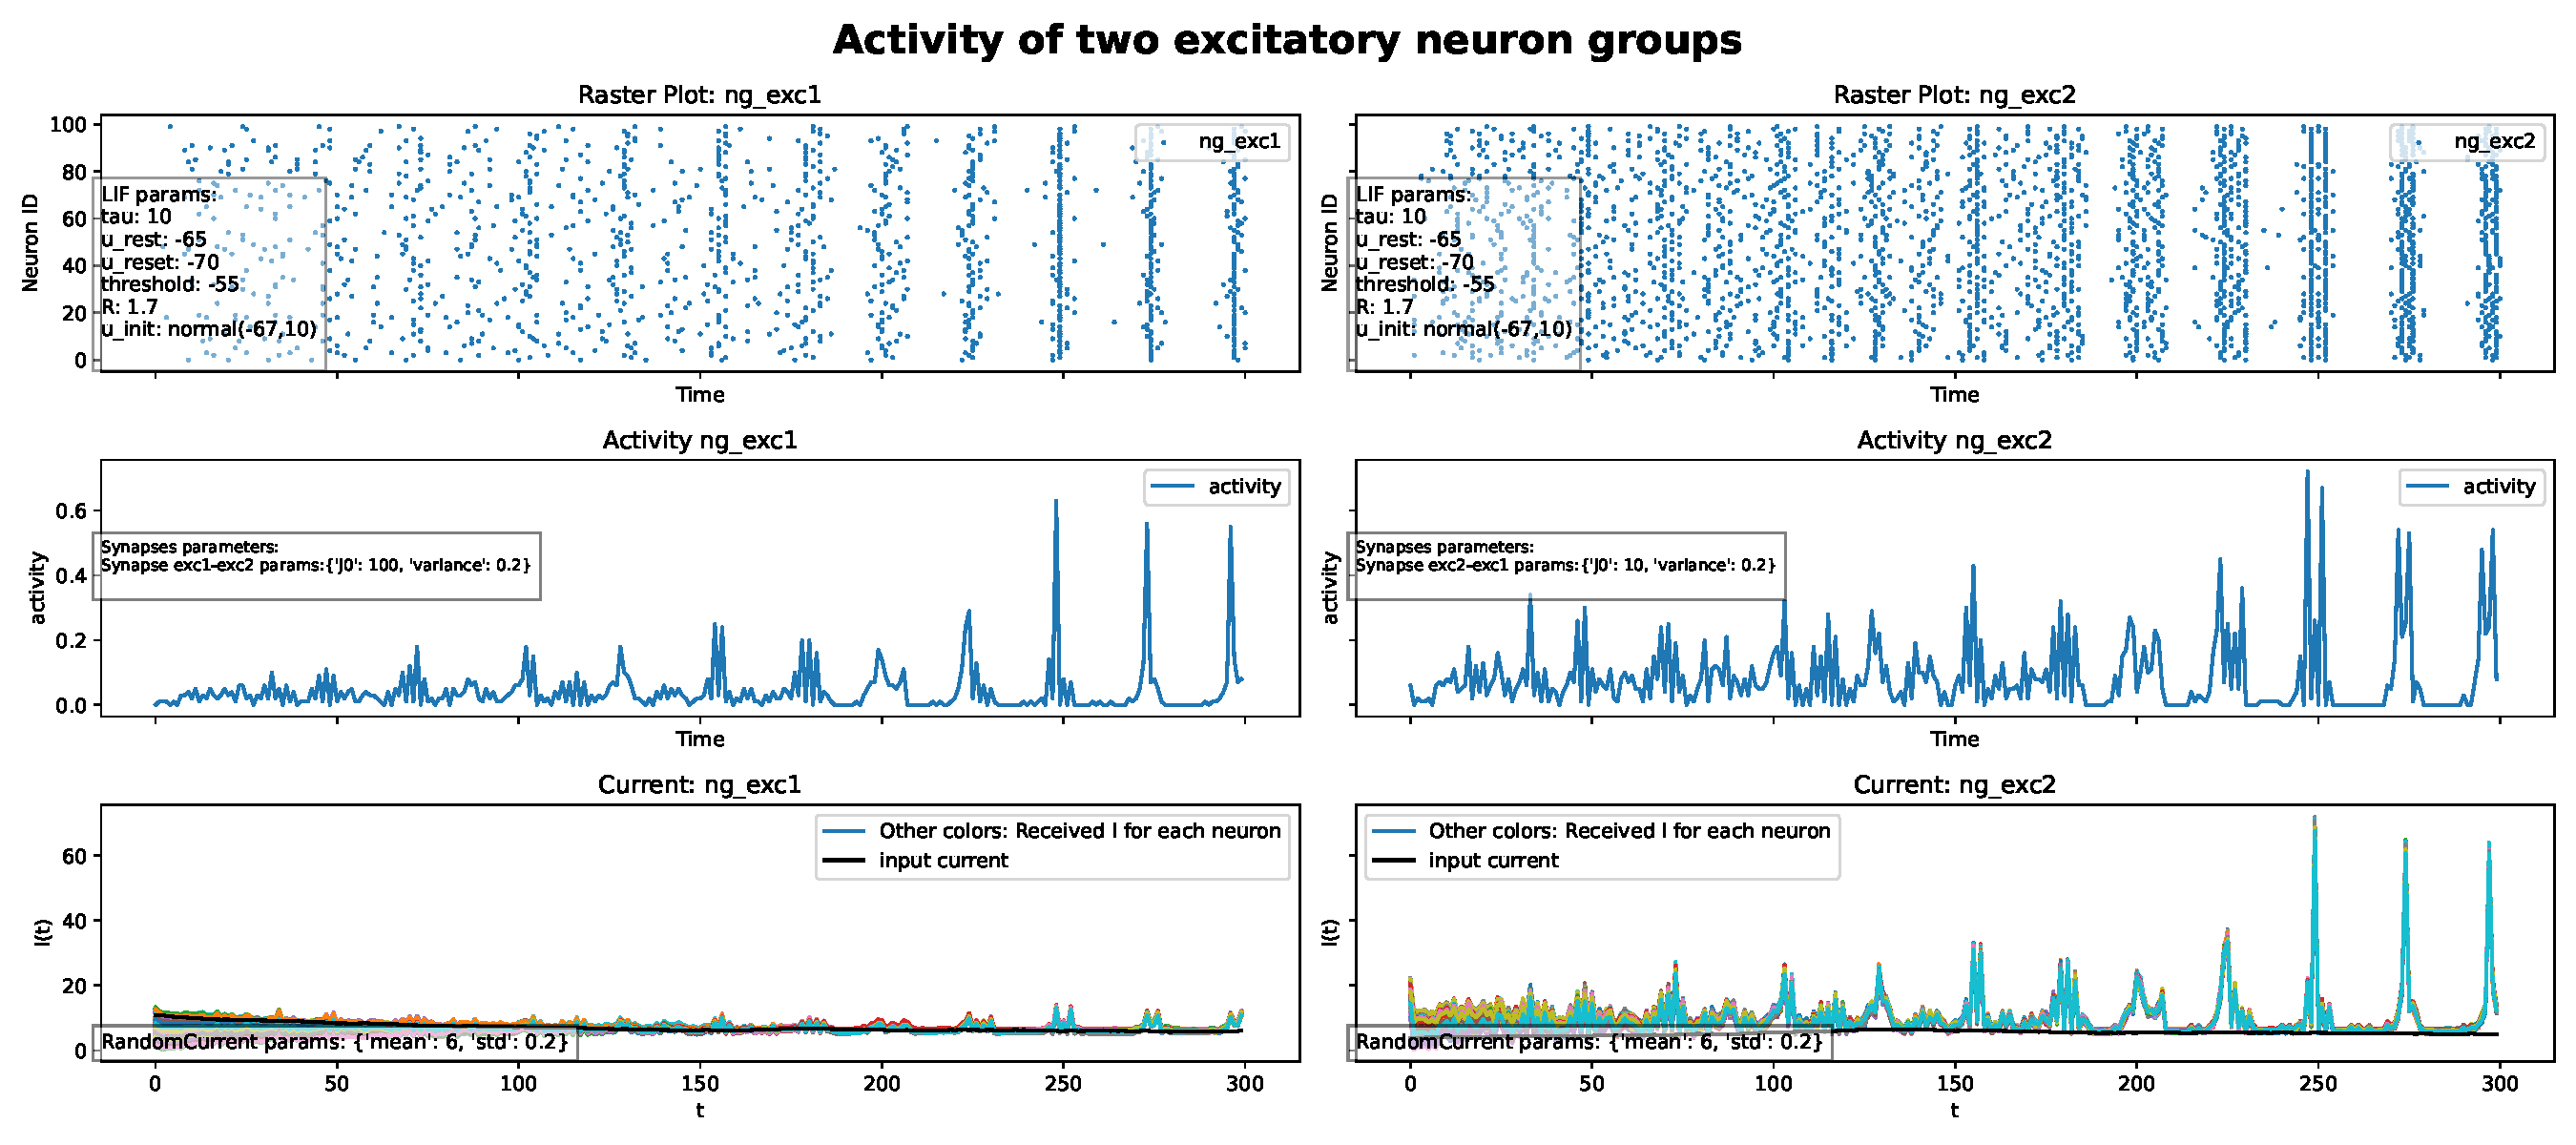
\includegraphics[width=0.9\textwidth]{plots/part2-two-ng-full-synapse-diff-j-rand-curr.pdf} 
                \caption{رفتار دو جمعیت نورونی با دو سیناپس و جریان تصادفی و $j_0$ متفاوت}
                \label{fig:part2-two-ng-full-synapse-diff-j-rand-curr}
            \end{figure}
        \paragraph*{پارامتر واریانس}
            حال با وزن های برابر با شکل 
            \ref{fig:part2-two-ng-full-synapse-noise-curr}
            مقادیر واریانس را افزایش داده و آن را تحلیل میکنیم.
            همانطور که در شکل 
            \ref{fig:part2-two-ng-full-synapse-high-variance-noise-curr}
            مشاهده می شود، افزایش واریانس به علت مشابهی که قبل تر نتیجه گرفته شد، تغییر چندانی در رفتار نورون با جریان های متفاوت ایجاد نمی کند.
            \begin{figure}[!ht]
                \centering
                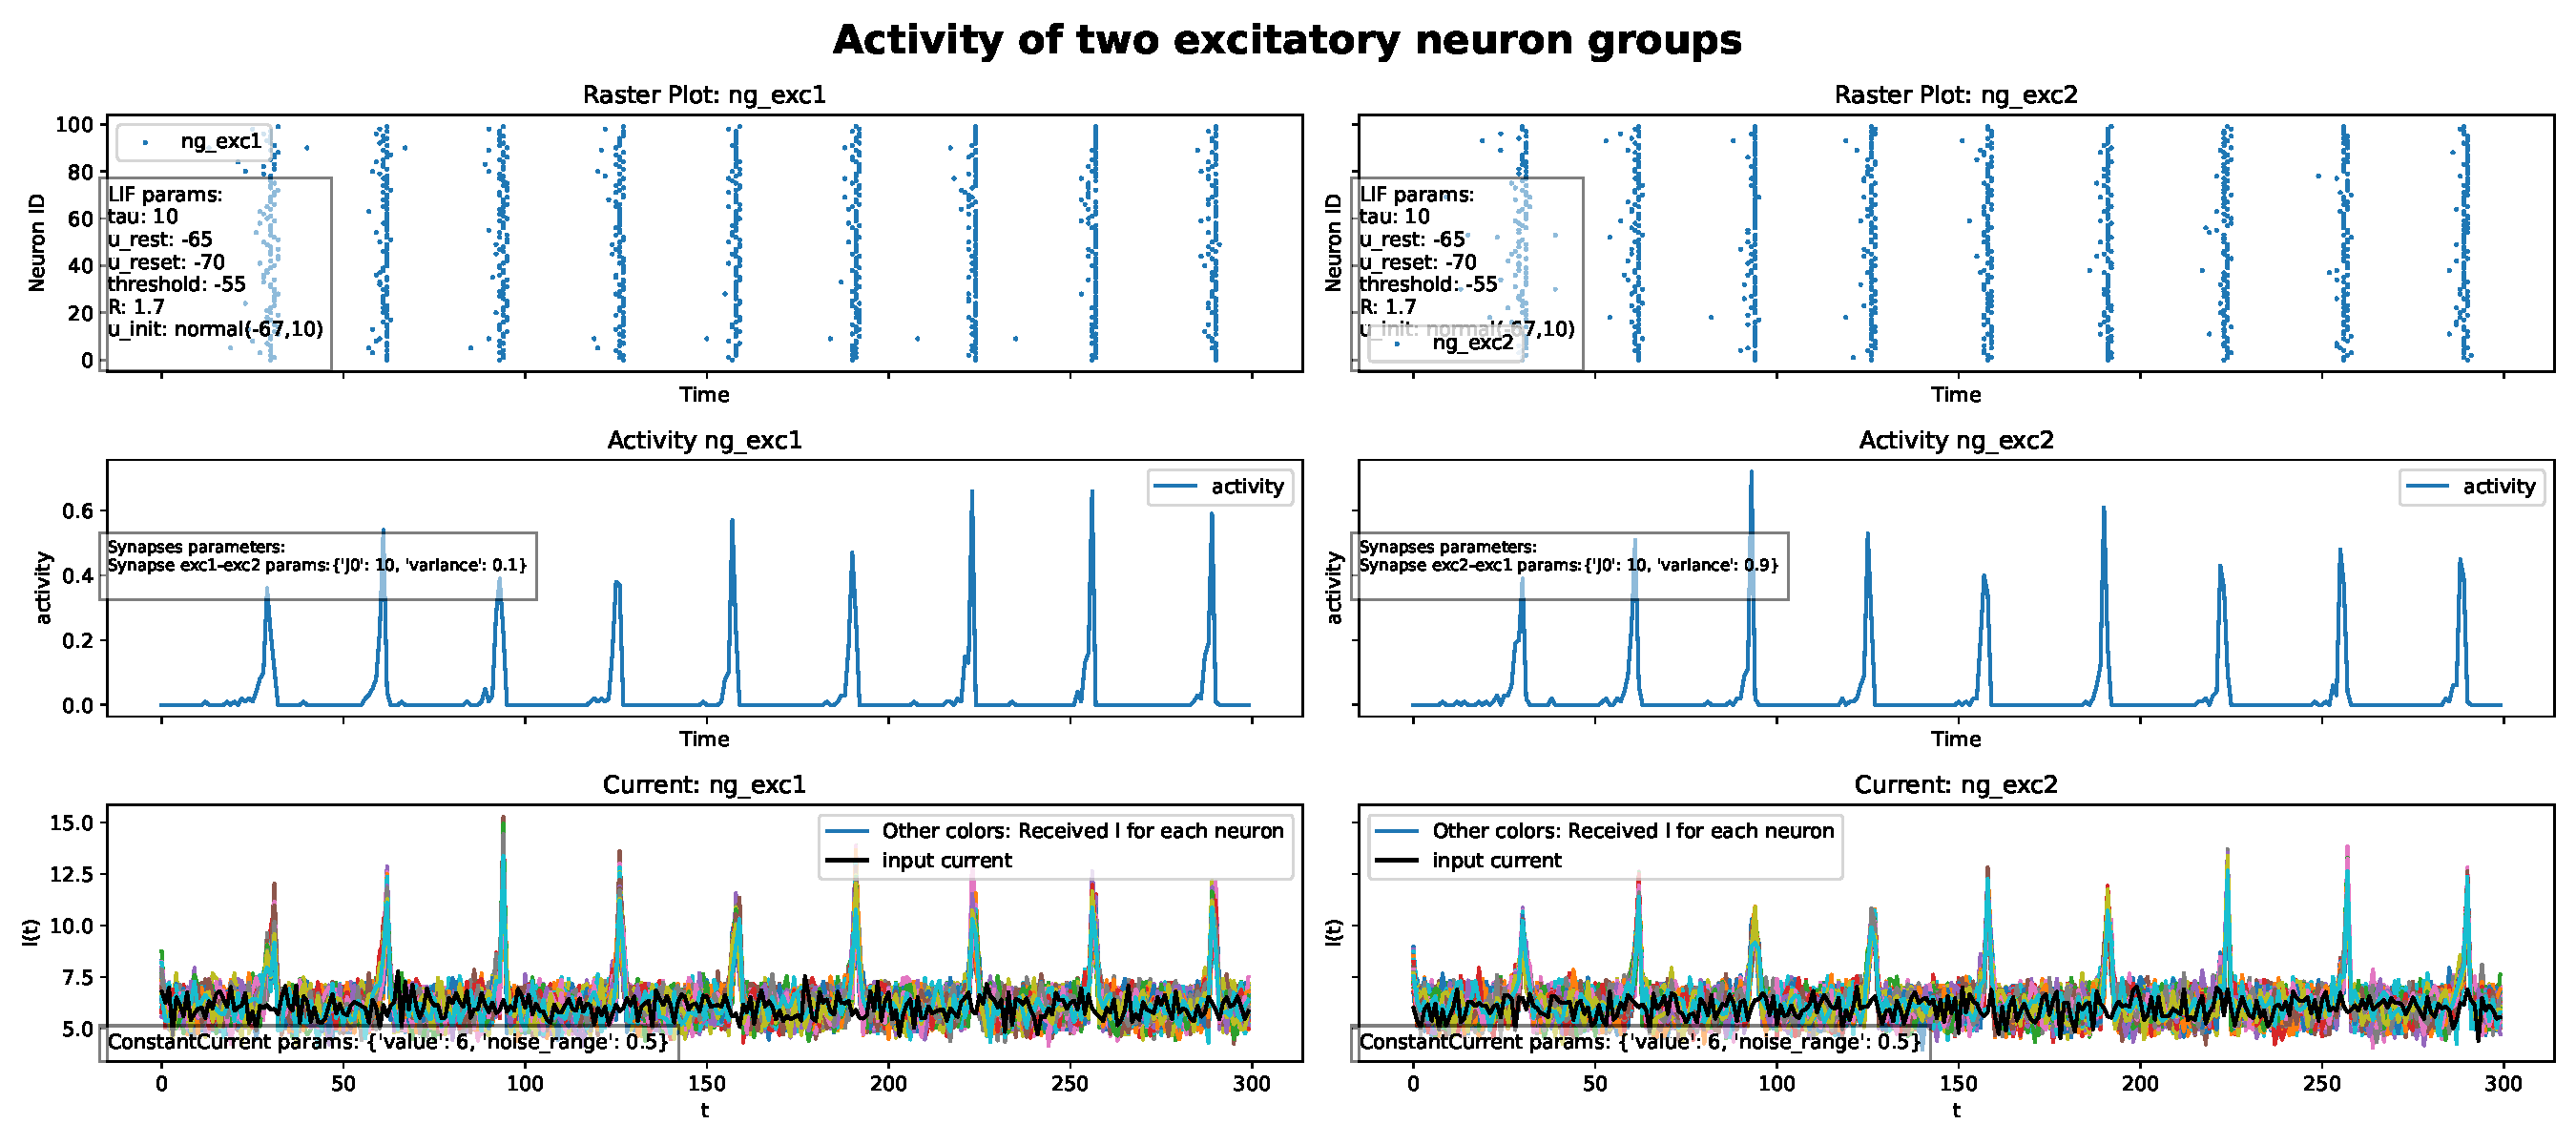
\includegraphics[width=0.9\textwidth]{plots/part2-two-ng-full-synapse-diff-variance-noise-curr.pdf} 
                \caption{رفتار دو جمعیت نورونی با دو سیناپس و جریان نویزی و واریانس زیاد}
                \label{fig:part2-two-ng-full-synapse-high-variance-noise-curr}
            \end{figure}

            مجددا مقدار واریانس ها را متفاوت در نظر میگریم و طبق شکل
            \ref{fig:part2-two-ng-full-synapse-diff-variance-rand-curr}
            مشاهده می شود که با واریانس متفاوت نیز تغییری در رفتار نورون ها اتفاق نمی افتد. طبعا نتیجه برای جریان تصادفی نیز به همین صورت است.
            \begin{figure}[!ht]
                \centering
                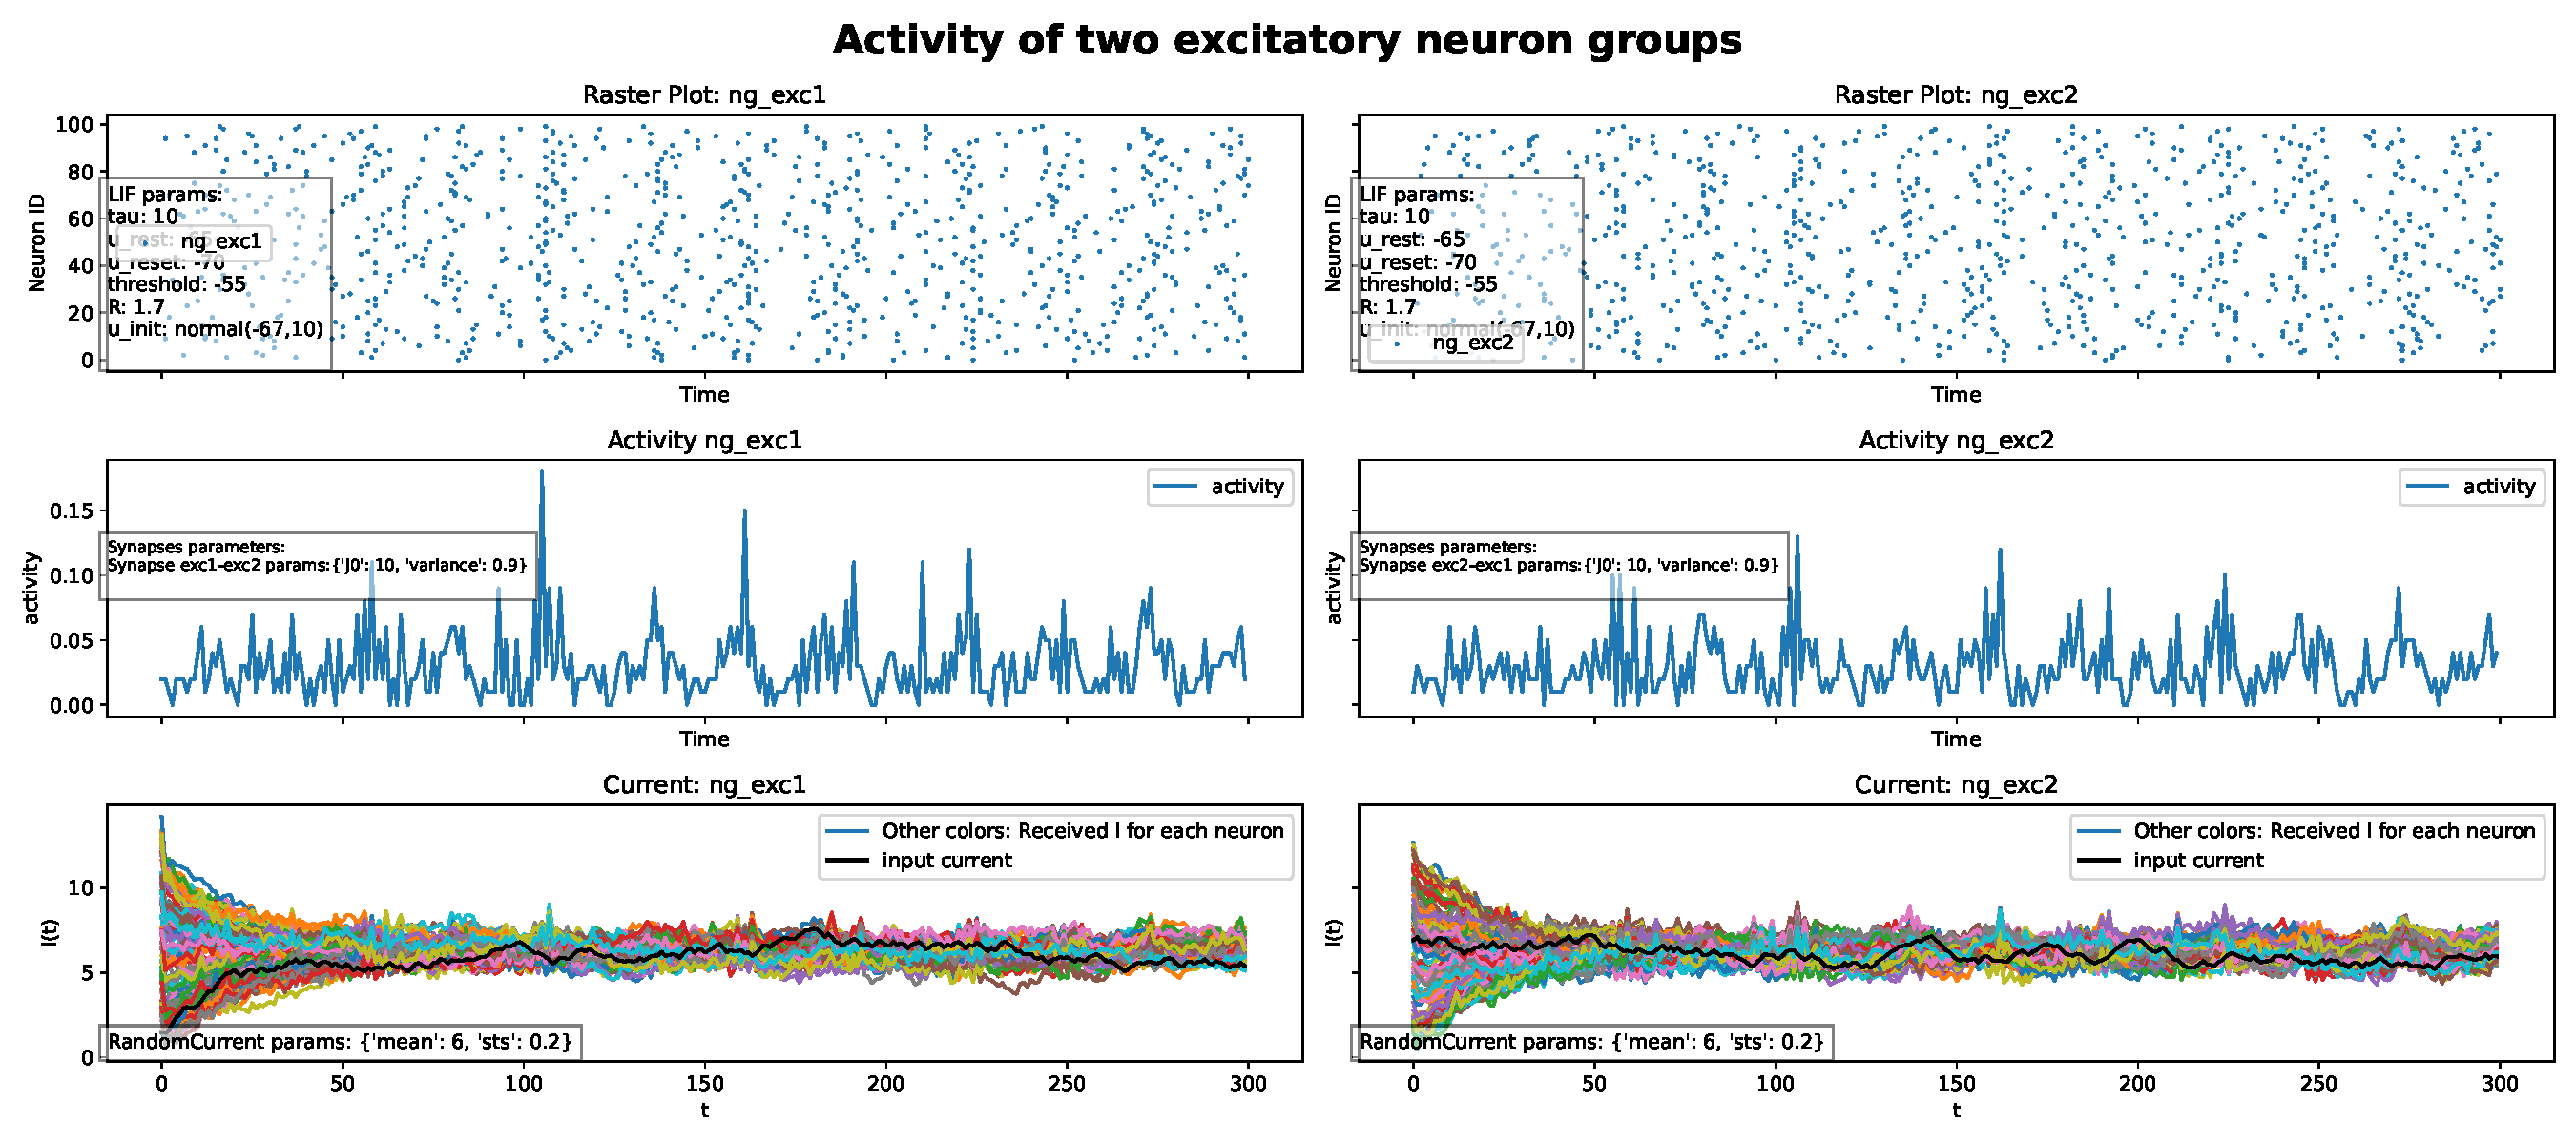
\includegraphics[width=0.9\textwidth]{plots/part2-two-ng-full-synapse-diff-variance-rand-curr.pdf} 
                \caption{رفتار دو جمعیت نورونی با دو سیناپس و جریان نویزی و واریانس متفاوت}
                \label{fig:part2-two-ng-full-synapse-diff-variance-rand-curr}
            \end{figure}
            همانطور که پیشتر گفته شد، اگر بخواهیم واریانس را به گونه ای تغییر دهیم که تاثیر قابل نمایشی داشته باشد، باید مقدار آن را زیادتر، مثلا ۱۰۰ بگیریم. مطابق شکل 
            \ref{fig:part2-two-ng-full-synapse-very-high-variance-noise-curr}
            تاثیر این مقدار نمایان است. این به این دلیل است که با خیلی زیاد شدن واریانس، بسیاری از وزن ها نیز آنقدر زیاد می شوند که تاثیر مجموع آن ها روی نورون های پس سیناپسی مشهود می شود.
            \begin{figure}[!ht]
                \centering
                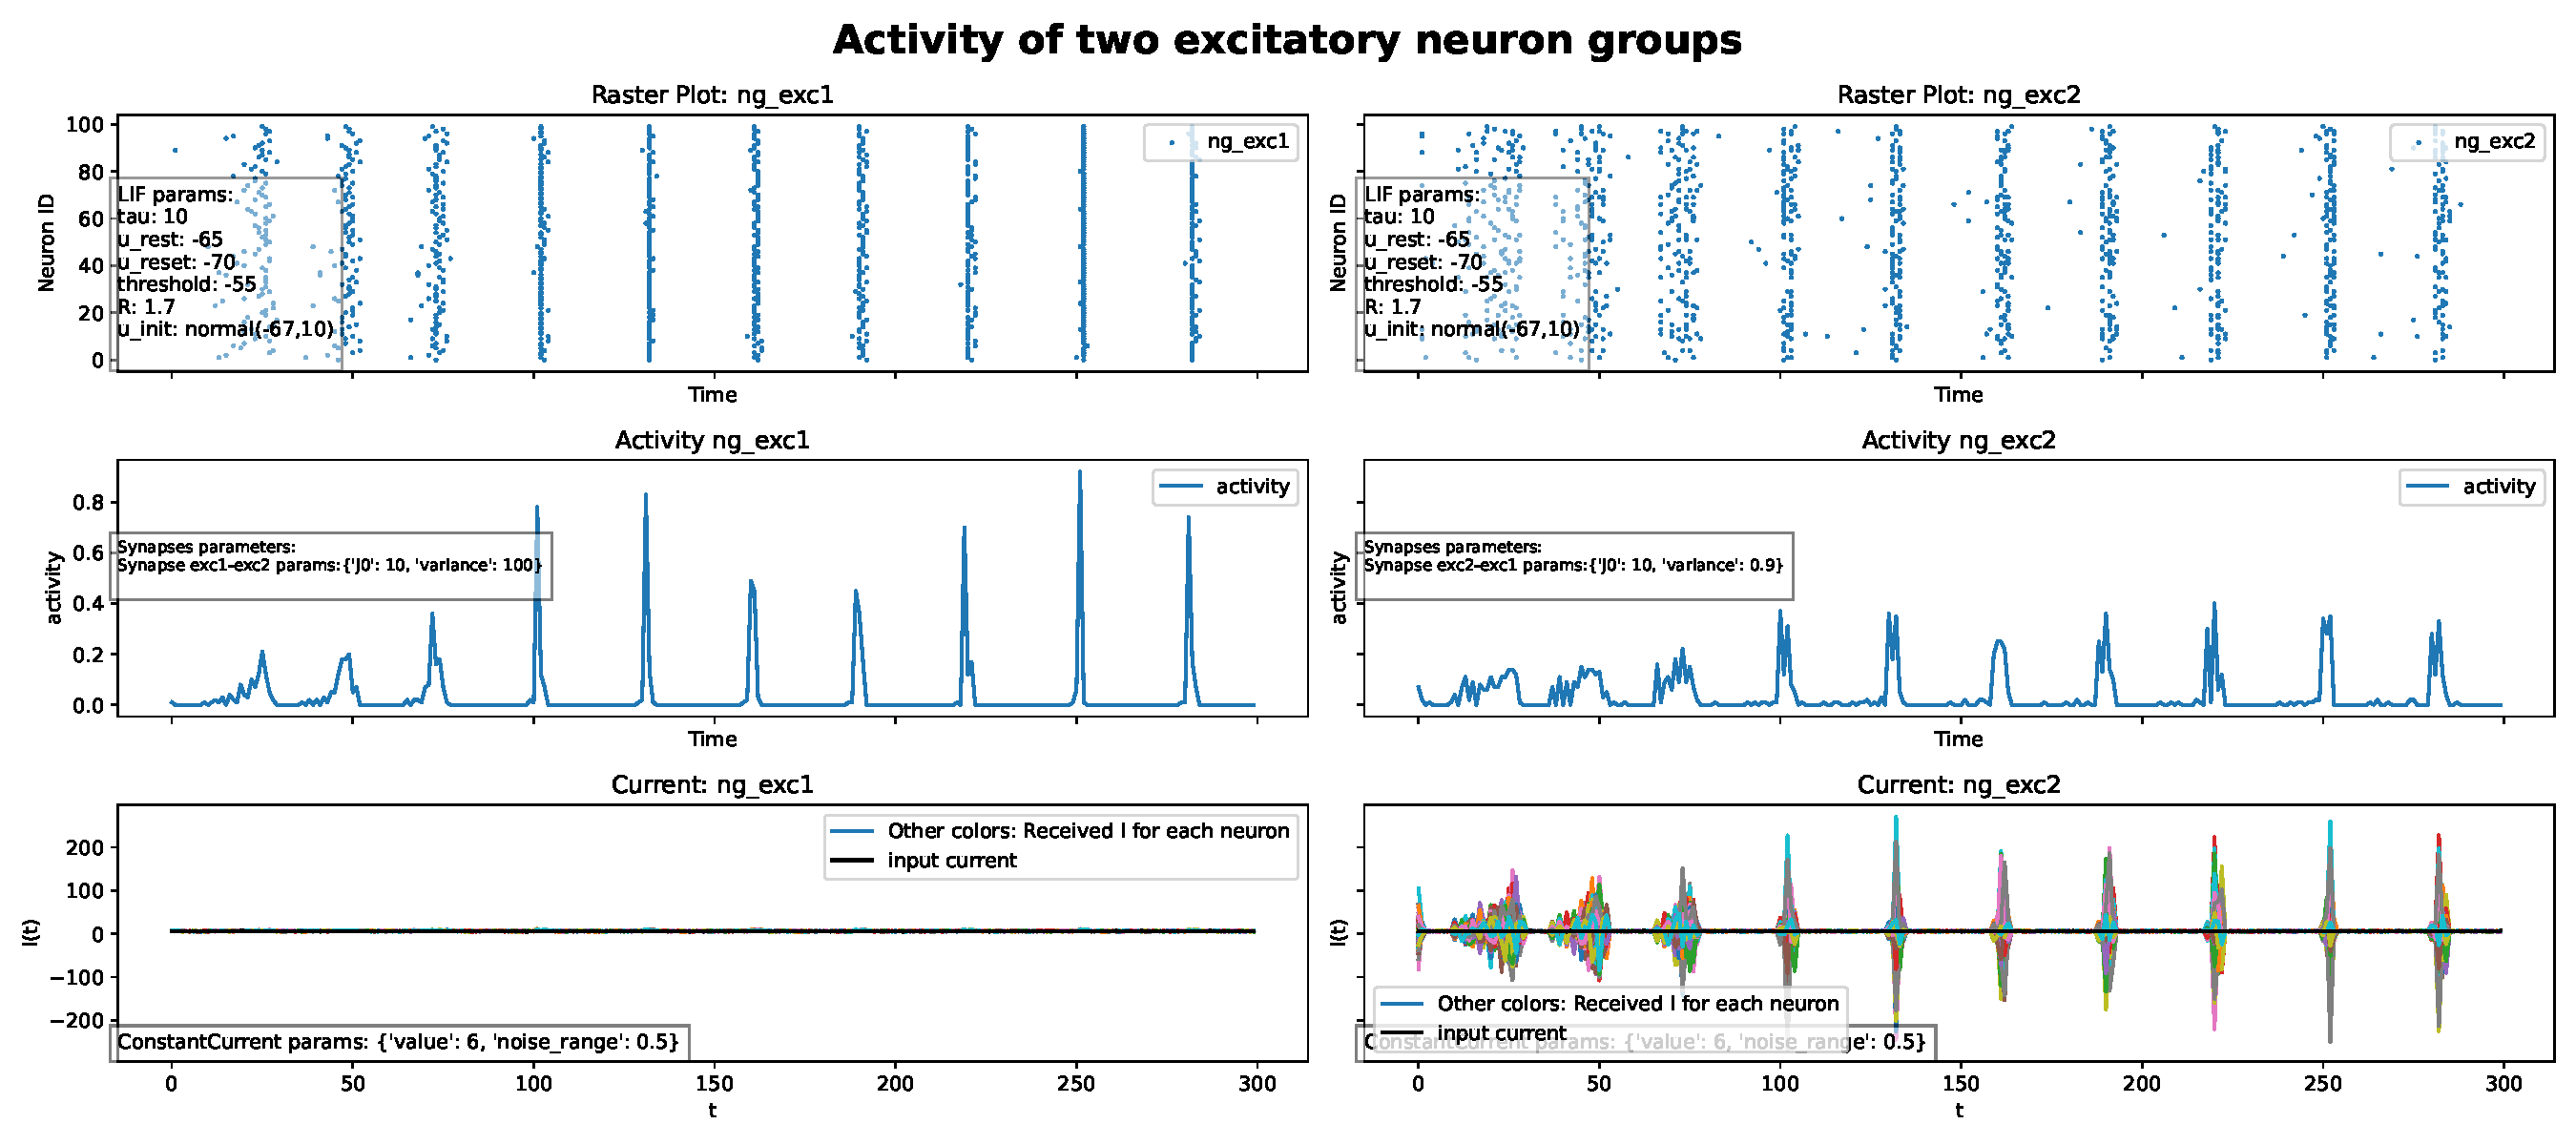
\includegraphics[width=0.9\textwidth]{plots/part2-two-ng-full-synapse-very-high-variance-noise-curr.pdf} 
                \caption{رفتار دو جمعیت نورونی با دو سیناپس و جریان نویزی و واریانس بسیار زیاد}
                \label{fig:part2-two-ng-full-synapse-very-high-variance-noise-curr}
            \end{figure}
            
            \paragraph*{تاثیر اندازه جمعیت}
            از آنجا که تنها دو جمعیت نورونی داریم، زیاد کردن هر دو جمعیت تاثیری مشابه تک جمعیت خواهد داشت، در نتیجه فقط حالتی را که یک جمعیت بزرگتر از دیگری است را آزمایش میکنیم. در این حالت نیز مشابه حالت های قبل میبینیم که فعالیت هر دو جمعیت پس از مدتی بیشتر می شود. هر چند میزان رشد جمعیت بزرگتر اندکی از جمعیت کوچکتر بیشتر است.
            (شکل \ref{fig:part2-two-ng-full-synapse-diff-size-noise-curr})
            \begin{figure}[!ht]
                \centering
                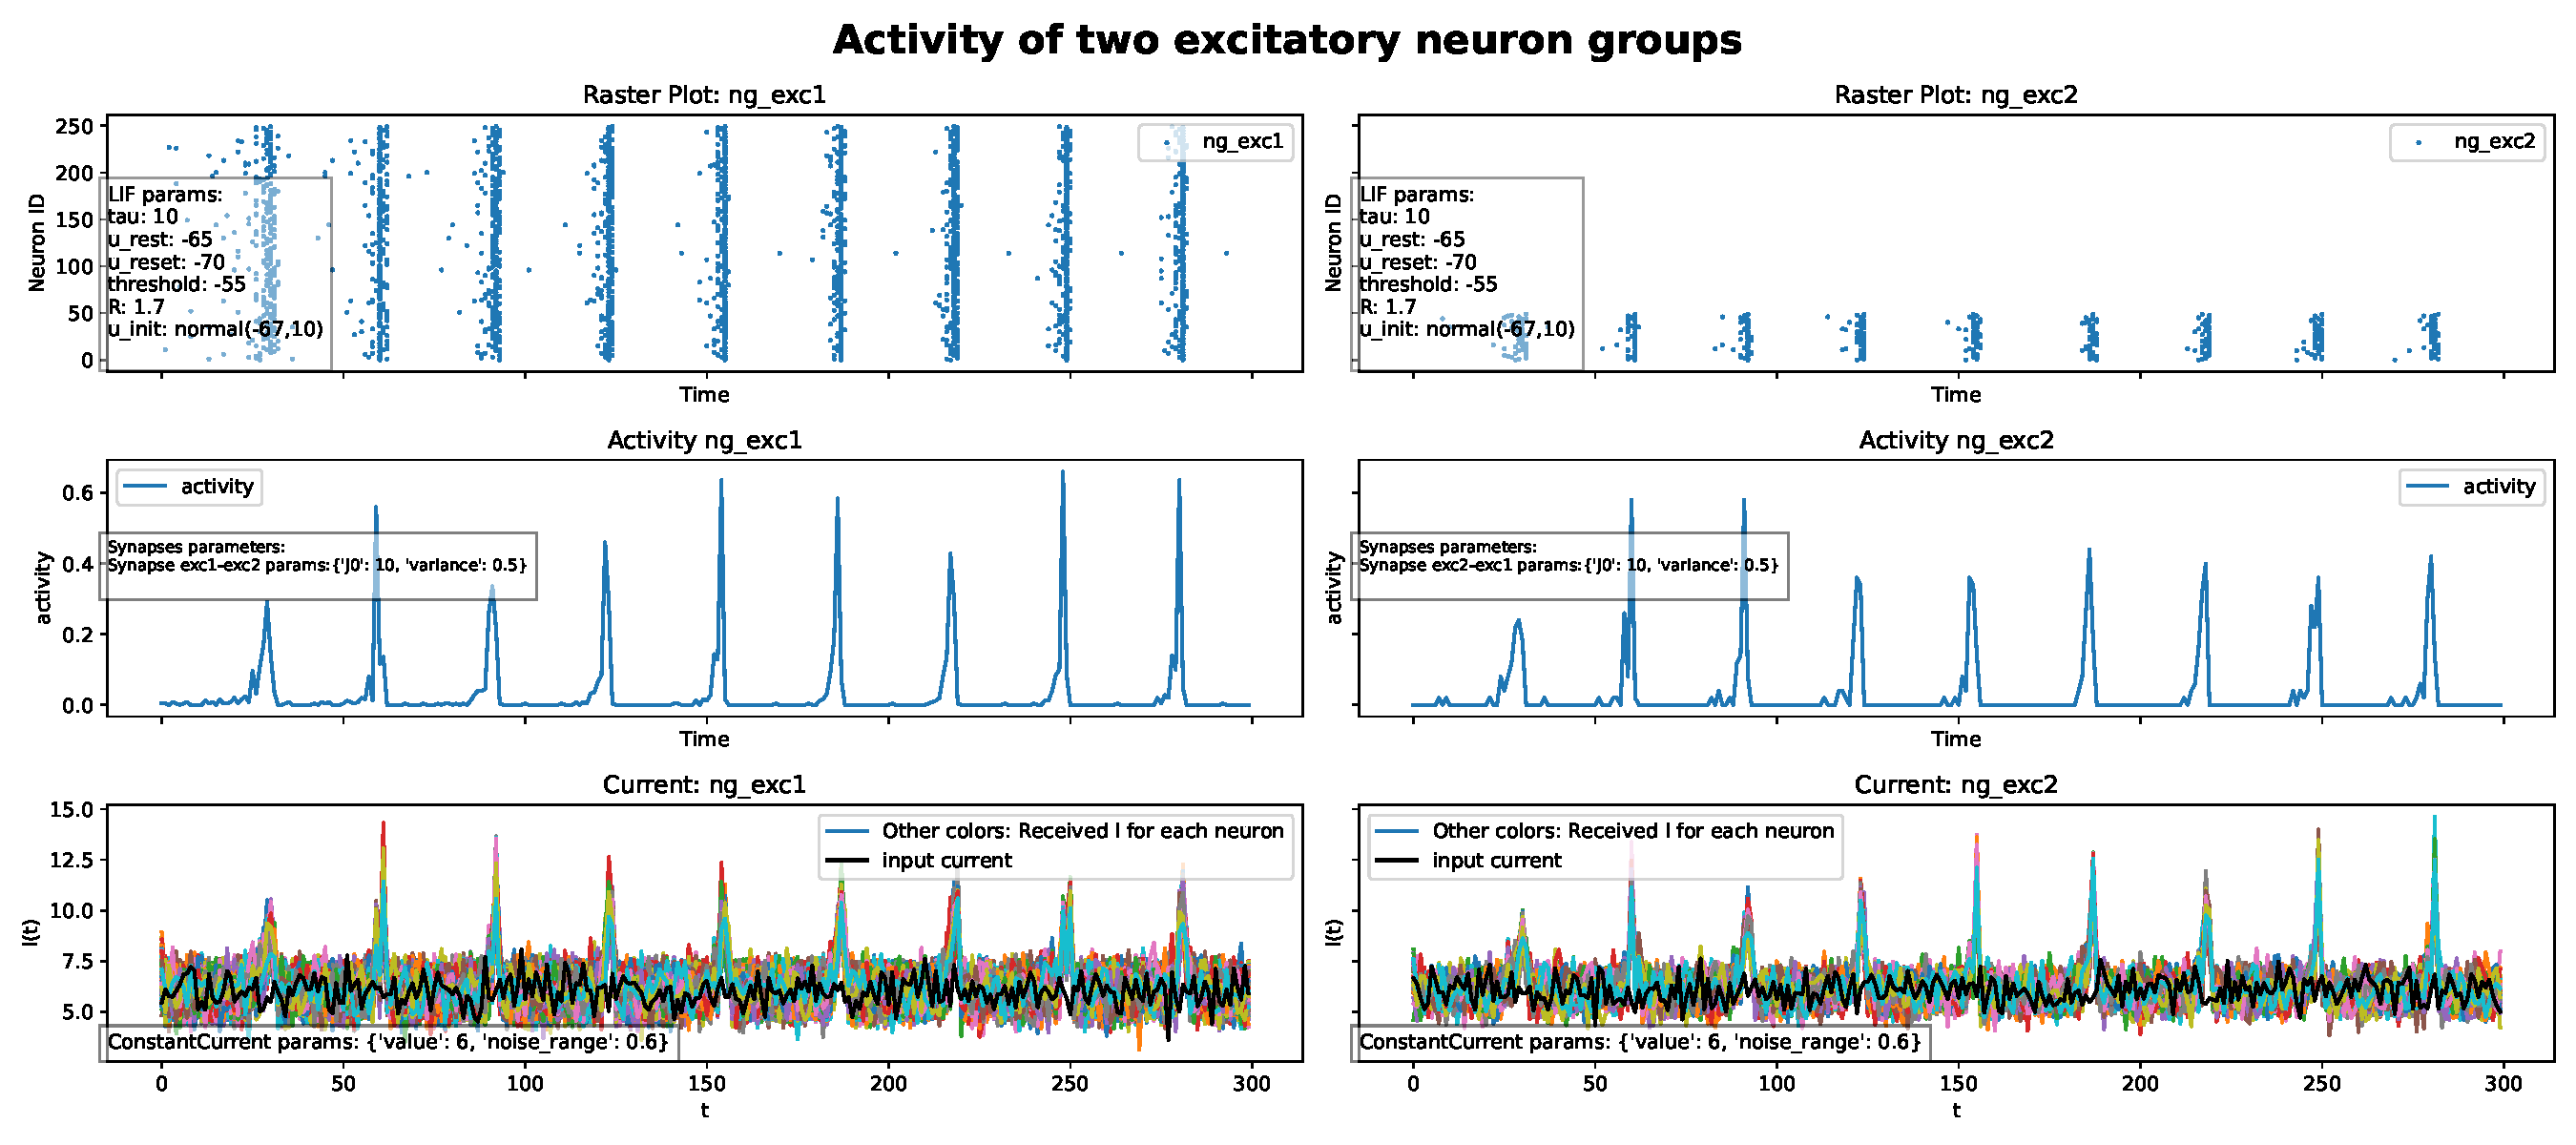
\includegraphics[width=0.9\textwidth]{plots/part2-two-ng-full-synapse-diff-size-noise-curr.pdf} 
                \caption{رفتار دو جمعیت نورونی با دو سیناپس و جریان نویزی و جمعیت متفاوت}
                \label{fig:part2-two-ng-full-synapse-diff-size-noise-curr}
            \end{figure}


    \subsection{الگوی ارتباط تصادفی با احتمال جفت شدن ثابت}
        در این قسمت به بررسی رفتار الگوی ارتباط تصادفی با احتمال جفت شدن ثابت می پردازیم. 

        از نظر تجربی، احتمال 
        $p$
        که یک نورون در داخل یک ستون قشر مغز، یک اتصال عملکردی به نورون دیگری در همان ستون برقرار کند، در محدوده 10 درصد است، هرچند این مقدار در بین لایه‌ها متفاوت است.

        در شبیه‌سازی‌ها، می‌توانیم یک احتمال اتصال 
        $p$ 
        را رفع کنیم و اتصالات را به‌طور تصادفی با احتمال 
        $p$ 
        از بین تمام اتصالات 
        $N^2$ 
        ممکن انتخاب کنیم. در این مورد، تعداد اتصال های ورودی پیش سیناپسی 
        $C_j$
        به یک نورون پس سیناپسی 
        $j$
        دارای مقدار میانگین 
        $\langle C_j = pN\rangle$
        است، اما بین یک نورون و نورون بعدی با واریانس 
        $p(1-p)N$ 
        در نوسان است.

        تا اینجای کار تاثیر بسیاری از پارامتر هایی که بررسی کردم شبیه تاثیر پارامتر های مشابه این الگو است. از این رو در این بخش تمرکزمان را روی پارامتر هایی میگذاریم که تاثیر متفاوت تری نسبت به حالت قبل دارند. در اینجا نیز مدل نورونی را مانند مدل های قبل درنظر میگیریم.
        \subsubsection*{بررسی رفتار یک جمعیت}
            برای شروع کار، بیایید رفتار یک جمعیت را با جریان ثابت، نویزی و تصادفی بررسی کنیم. همانطور که از شکل 
            \ref{fig:part2-one-ng-prob-synapse-diff-curr}
            بر می‌آید، رفتار نورون همانند الگوی ارتباط قبلی بوده و پس از مدتی، پراکندگی زمان ضربه زدن نورون ها کمتر شده و فعالیت رفته رفته بیشتر می شود و این بیشتر شدن به ترتیب نمودار ها از سمت چپ به راست سرعت کمتری دارد. دلیل این امر نیز مشابه الگو های قبل، زیاد شدن جریان سیناپسی است.
            \begin{figure}[!ht]
                \centering
                \includegraphics[width=0.9\textwidth]{plots/part2-one-ng-prob-synapse-diff-curr.pdf} 
                \caption{رفتار تک جمعیت های نورونی با سیناپس داخلی و جریان ثابت، نویزی و تصادفی}
                \label{fig:part2-one-ng-prob-synapse-diff-curr}
            \end{figure}
            
            حال به سراغ آزمایش پارامترها میرویم. پارامتر 
            $j_0$ 
            تاثیری مشابه الگوی قبلی دارد و خیلی روی آن تمرکز نمیکنیم
            \paragraph*{پارامتر $j_0$}
                همانطور که در شکل
                \ref{fig:part2-one-ng-prob-synapse-diff-j-rand-curr}
                مشاهده می شود، افزایش مقدار 
                $j_0$ 
                باعث کاهش پراکندگی زمان ضربه زدن نورون ها و افزایش فعالیت جمعیت می شود. همانطور که از شکل نیز بر می آید، دلیل این امر مانند الگوی گذشته، افزایش جریان سیناپسی و درنتیجه افزایش فعالیت جمعیت است.
                \begin{figure}[!ht]
                    \centering
                    \includegraphics[width=0.9\textwidth]{plots/part2-one-ng-prob-synapse-diff-j-rand-curr.pdf} 
                    \caption{رفتار تک جمعیت های نورونی با سیناپس داخلی و جریان تصادفی $j_0$ متفاوت}
                    \label{fig:part2-one-ng-prob-synapse-diff-j-rand-curr}
                \end{figure}

            
            \paragraph*{پارامتر واریانس}
                برای درک بهتر تاثیر این پارامتر، ابتدا یک جریان تصادفی ولی یکسان برای همه نورون ها به جمعیت میدهیم.
                در این الگو طبق شکل 
                \ref{fig:part2-one-ng-prob-synapse-diff-variance-same-rand-curr}
                ملاحظه میکنیم که تغییر در واریانس میتواند مقدار کمی رفتار جمعیت را تغییر دهد. بدین صورت که با افزایش واریانس از 
                $0.2$ 
                تا
                $0.6$ 
                وزن های اولیه، باعث می شود فعالیت جمعیت کاهش یابد. اگر آزمایش را با همین پارامتر ها ولی با جریان تصادفی غیر یکسان اجرا کنیم، میبینیم که تاثیر واریانس کمرنگ تر می شود.
                (شکل \ref{fig:part2-one-ng-prob-synapse-diff-variance-rand-curr})
                \begin{figure}[!ht]
                    \centering
                    \includegraphics[width=0.9\textwidth]{plots/part2-one-ng-prob-synapse-diff-variance-same-rand-curr.pdf} 
                    \caption{رفتار تک جمعیت های نورونی با سیناپس داخلی و جریان تصادفی یکسان و واریانس متفاوت}
                    \label{fig:part2-one-ng-prob-synapse-diff-variance-same-rand-curr}
                \end{figure}
                \begin{figure}[!ht]
                    \centering
                    \includegraphics[width=0.9\textwidth]{plots/part2-one-ng-prob-synapse-diff-variance-rand-curr.pdf} 
                    \caption{رفتار تک جمعیت های نورونی با سیناپس داخلی و جریان تصادفی و واریانس متفاوت}
                    \label{fig:part2-one-ng-prob-synapse-diff-variance-rand-curr}
                \end{figure}
            
            \paragraph*{پارامتر $p$}
                حال نوبت به پارامتر جدید این الگو می رسد. این پارامتر  بیان می دارد که هر نورون با چه احتمالی با نورون های دیگر در ارتباط باشد. در آزمایش اول نیز همانند قبل، ابتدا جمعیت را با جریان تصادفی یکسان آزمایش میکنیم. طبق شکل 
                \ref{fig:part2-one-ng-prob-synapse-diff-p-same-noise-curr}
                مشاهده می شود که با افزایش 
                $p$ 
                فعالیت جمعیت نیز افزایش می یابد، این به این دلیل می تواند باشد که افزایش 
                $p$ 
                سبب افزایش ارتباطات و درنتیجه افزایش جریان سیناپسی و در نهایت افزایش فعالیت نورونی شود.
                \begin{figure}[!ht]
                    \centering
                    \includegraphics[width=0.9\textwidth]{plots/part2-one-ng-prob-synapse-diff-p-same-noise-curr.pdf} 
                    \caption{رفتار تک جمعیت های نورونی با سیناپس داخلی و جریان نویزی یکسان و $p$ متفاوت}
                    \label{fig:part2-one-ng-prob-synapse-diff-p-same-noise-curr}
                \end{figure}
                تکرار آزمایش با جریان ثابت نویزی نیز نتیجه ای مشابه به ما میدهد.
                (شکل \ref{fig:part2-one-ng-prob-synapse-diff-p-noise-curr})
                \begin{figure}[!ht]
                    \centering
                    \includegraphics[width=0.9\textwidth]{plots/part2-one-ng-prob-synapse-diff-p-noise-curr.pdf} 
                    \caption{رفتار تک جمعیت های نورونی با سیناپس داخلی و جریان نویزی غیر یکسان و $p$ متفاوت}
                    \label{fig:part2-one-ng-prob-synapse-diff-p-noise-curr}
                \end{figure}

                اگر جریان ورودی تصادفی غیر یکسان را در نظر بگیریم، مشاهده میکنیم که هر چند تاثیر این تفاوت کمرنگ تر میشود ولی هنوز می توان افزایش کلی فعالیت جمعیت در طول شبیه سازی را مشاهده کرد.
                (شکل \ref{fig:part2-one-ng-prob-synapse-diff-p-rand-curr})
                \begin{figure}[!ht]
                    \centering
                    \includegraphics[width=0.9\textwidth]{plots/part2-one-ng-prob-synapse-diff-p-rand-curr.pdf} 
                    \caption{رفتار تک جمعیت های نورونی با سیناپس داخلی و جریان تصادفی و $p$ متفاوت}
                    \label{fig:part2-one-ng-prob-synapse-diff-p-rand-curr}
                \end{figure}

        \subsubsection*{بررسی رفتار دو جمعیت}
            حال نوبت به بررسی رفتار دو جمعیت با سیناپسی با این الگو می رسد. برای شروع، ابتدا دو جمعیت نورونی ایجاد کرده و به یکدیگر سیناپس میزنیم و برای هر دو یک جریان ثابت در نظر میگیریم. اضافه کردن سیناپس داخلی برای هر یک را، به بخش سوم می سپاریم. رفتار جمعیت ها مشابه شکل 
            \ref{fig:part2-two-ng-prob-synapse-const-curr}
            می شود که در آن نکته جدیدی مشاهده نمیکنیم. جریان ثابت باعث ضربه زدن نورون ها می شود و در لحظه هایی که همه نورون ها در یک جمعیت ضربه می زنند، فعالیت نورونی نیز افزایش می یابد. به دلیل اینکه تاثیر سیناپس ها در یک لحظه است، این افزایش ناگهانی تاثیر چندانی روی نورون های مقصد نمیگذارد. تکرار آزمایش با جریان تصادفی نیز الگوی خاصی ندارد.
            (شکل \ref{fig:part2-two-ng-prob-synapse-rand-curr})
            پس به سراغ آزمایش پارامتر های مختلف می رویم.
            \begin{figure}[!ht]
                \centering
                \includegraphics[width=0.9\textwidth]{plots/part2-two-ng-prob-synapse-const-curr.pdf} 
                \caption{رفتار دو جمعیت نورونی با سیناپس و جریان ثابت}
                \label{fig:part2-two-ng-prob-synapse-const-curr}
            \end{figure}
            \begin{figure}[!ht]
                \centering
                \includegraphics[width=0.9\textwidth]{plots/part2-two-ng-prob-synapse-rand-curr.pdf} 
                \caption{رفتار دو جمعیت نورونی با سیناپس و جریان تصادفی}
                \label{fig:part2-two-ng-prob-synapse-rand-curr}
            \end{figure}

            \paragraph*{پارامتر $j_0$}
                حال دو جمعیت بالا را انتخاب کرده، و تاثیر افزایش 
                $j_0$ 
                را روی آن ها میبینیم. در شکل 
                \ref{fig:part2-two-ng-prob-synapse-high-j}
                مشاهده میکنیم که با افزایش
                $j_0$ 
                نسبت به شکل 
                \ref{fig:part2-two-ng-prob-synapse-rand-curr}
                فعالیت نورون ها افزایش می یابد. دلیل این امر، افزایش جریان سیناپسی و درنتیجه افزایش جریان ورودی به نورون ها است.
                \begin{figure}[!ht]
                    \centering
                    \includegraphics[width=0.9\textwidth]{plots/part2-two-ng-prob-synapse-high-j.pdf} 
                    \caption{رفتار دو جمعیت نورونی با سیناپس و جریان تصادفی در اثر افزایش $j_0$}
                    \label{fig:part2-two-ng-prob-synapse-high-j}
                \end{figure}

                حال اگر وزن های سیناپسی از جمعیت ۱ به ۲ نسبت به دیگری بیشتر باشد چه اتفاقی می افتد؟ طبق شکل
                \ref{fig:part2-two-ng-prob-synapse-rand-curr-diff-j}
                ملاحظه می شود که فعالیت هر دو جمعیت نسبت به نمودار
                \ref{fig:part2-two-ng-prob-synapse-rand-curr} 
                افزایش می یابد و فعالیت جمعیت دوم بیشتر از جمعیت اول می شود.
                \begin{figure}[!ht]
                    \centering
                    \includegraphics[width=0.9\textwidth]{plots/part2-two-ng-prob-synapse-rand-curr-diff-j.pdf} 
                    \caption{رفتار دو جمعیت نورونی با سیناپس و جریان تصادفی در اثر تفاوت $j_0$}
                    \label{fig:part2-two-ng-prob-synapse-rand-curr-diff-j}
                \end{figure}

                از آنجا که انتخاب جریان تصادفی یکسان نیز تاثیری مشابه دارد، از آوردن نمودار آن خودداری می شود. به طور کلی افزایش 
                $j_0$ 
                باعث افزایش فعالیت جمعیت مقصد می شود. حال انتخاب جریان ثابت، نویزی، تصادفی صرفا به ترتیب میزان پراکندگی و تصادفی بودن زمان ضربه زدن نورون ها را بیشتر می کند. همچنین غیریکسان بودن جریان نورون ها نسبت به یکسان بودن نیز تاثیر مشابهی دارد.

                \paragraph*{پارامتر واریانس}
                    با افزایش واریانس هر دو سیناپس شروع می کنیم. همانطور که از شکل
                    \ref{fig:part2-two-ng-prob-synapse-rand-curr-high-variance}
                    نیز بر می آید، افزایش واریانس همانند قبل، نسبت به نمودار
                    \ref{fig:part2-two-ng-prob-synapse-rand-curr}
                    تاثیر بسزایی روی رفتار کلی جمعیت ها نمیگذارد و فقط اندکی فعالیت ان ها را کاهش می دهد.
                    \begin{figure}[!ht]
                        \centering
                        \includegraphics[width=0.9\textwidth]{plots/part2-two-ng-prob-synapse-rand-curr-high-variance.pdf} 
                        \caption{رفتار دو جمعیت نورونی با سیناپس و جریان تصادفی در اثر افزایش واریانس}
                        \label{fig:part2-two-ng-prob-synapse-rand-curr-high-variance}
                    \end{figure}
                    این موضوع برای تفاوت واریانس دو سیناپس نیز صدق می کند.

                \paragraph*{پارامتر $p$}
                    مجددا به بررسی پارامتر جدید این الگو میرسیم. ابتدا آزمایش میکنیم که با افزایش این پارامتر، چه تغییری در رفتار دو جمعیت ایجاد خواهد شد. همانطور که از شکل 
                    \ref{fig:part2-two-ng-prob-synapse-high-p-rand-curr}
                    بر می آید، افزایش 
                    $p$ 
                    نسبت به شکل 
                    \ref{fig:part2-two-ng-prob-synapse-rand-curr}
                    از 
                    $0.1$ 
                    به 
                    $0.75$ 
                    باعث افزایش فعالیت نسبی جمعیت ها می شود که مشابه حالت های قبل، دلیل آن افزایش جریان سیناپسی و سپس جریان دریافتی به نورون است.
                    \begin{figure}[!ht]
                        \centering
                        \includegraphics[width=0.9\textwidth]{plots/part2-two-ng-prob-synapse-high-p-rand-curr.pdf} 
                        \caption{رفتار دو جمعیت نورونی با سیناپس و جریان تصادفی در اثر افزایش $p$}
                        \label{fig:part2-two-ng-prob-synapse-high-p-rand-curr}
                    \end{figure}
                    
                    حال اگر مقدار پارامتر 
                    $p$ 
                    در سیناپس جمعیت ۱ به ۲ را نیز افزایش دهیم، مطابق شکل
                    \ref{fig:part2-two-ng-prob-synapse-diff-p-rand-curr}
                    مشاهده میکنیم که فعالیت کلی جمعیت ها کمی افزایش یافته و فعالیت جمعیت ۲ نیز کمی بیشتر از جمعیت ۱ می شود.
                    \begin{figure}[!ht]
                        \centering
                        \includegraphics[width=0.9\textwidth]{plots/part2-two-ng-prob-synapse-diff-p-rand-curr.pdf} 
                        \caption{رفتار دو جمعیت نورونی با سیناپس و جریان تصادفی در اثر تفاوت $p$}
                        \label{fig:part2-two-ng-prob-synapse-diff-p-rand-curr}
                    \end{figure}
    
    \subsection{الگوی ارتباط تصادفی با تعداد ثابت نورون پیش سیناپسی }
        نوبت به آخرین الگوی ارتباطی از این بخش می رسد. در این قسمت به آزمایش ارتباط تصادفی با تعداد ثابت نورون پیش سیناپسی بین جمعیت های نورونی می پردازیم. از آنجا که این الگو شباهت با الگوی قبل دارد، تاثیر بعضی پارامتر ها مشابه یکدگیر است. در نتیجه از آوردن نمودار های تکراری جلوگیری می شود.

        تعداد سیناپس ها بر روی دندریت های یک نورون هرمی منفرد در محدوده چند هزار تخمین زده می شود. بنابراین، وقتی شبکه‌های صد هزار نورون یا میلیون‌ها نورون را شبیه‌سازی می‌کنیم، رویکرد مدل‌سازی مبتنی بر احتمال اتصال ثابت در محدوده 10 درصد نمی‌تواند درست باشد. علاوه بر این، در حیوانی که در یک آزمایش شرکت می کند، همه نورون ها به طور همزمان فعال نخواهند بود. بلکه فقط چند زیرگروه فعال خواهند بود که ترکیب آنها به شرایط تحریک و وظیفه بستگی دارد. به عبارت دیگر، تعداد ورودی هایی که به یک نورون منفرد همگرا می شوند ممکن است بسیار کوچکتر از هزار باشد.

        با روش زیر می توانیم یک شبکه تصادفی با تعداد ورودی ثابت بسازیم. ما یک نورون  
        $j=1,2,3,...,N$
        را پس از دیگری انتخاب می کنیم و به طور تصادفی جفت های پیش سیناپسی آن را انتخاب می کنیم.
        را ببینید. هر زمان که اندازه شبکه 
        $N$
        بسیار بزرگتر از 
        $C$ 
        باشد، ورودی های یک نورون معین را می توان به عنوان نمونه های تصادفی از فعالیت شبکه فعلی در نظر گرفت. بدون مقیاس بندی اتصالات با اندازه جمعیت 
        $N$ 
        لازم نیست. \cite{Neuronal-Dynamics}

        \subsubsection*{بررسی رفتار یک جمعیت}
            مثل همیشه، ابتدا با یک جمعیت ساده با جریان ثابت و سیناپس داخل شروع میکنیم و سپس آزمایش های بعدی را با آن مقایسه می کنیم.
            (شکل \ref{fig:part2-one-ng-fixed-synapse-const-curr})
            \begin{figure}[!ht]
                \centering
                \includegraphics[width=0.9\textwidth]{plots/part2-one-ng-fixed-synapse-const-curr.pdf} 
                \caption{رفتار تک جمعیت نورونی با سیناپس و جریان ثابت}
                \label{fig:part2-one-ng-fixed-synapse-const-curr}
            \end{figure}
            ملاحظه میکنیم که مانند گذشته، فعالیت جمعیت به دلیل افزایش جریان سیناپسی، رفته رفته بیشتر می شود. نمودار با جریان تصادفی نیز در شکل
            \ref{fig:part2-one-ng-fixed-synapse-rand-curr}
            آمده است که میبینیم پراکندگی زمان ضربه زدن نورون ها را حتی با نویز کم خیلی افزایش داده است.
            \begin{figure}[!ht]
                \centering
                \includegraphics[width=0.9\textwidth]{plots/part2-one-ng-fixed-synapse-rand-curr.pdf} 
                \caption{رفتار تک جمعیت نورونی با سیناپس و جریان تصادفی}
                \label{fig:part2-one-ng-fixed-synapse-rand-curr}
            \end{figure}

            \paragraph*{پارامتر $j_0$}
                ابتدا، رفتار جمعیت را با یک جریان نویزی به ازای مقادیر مختلف 
                $j_0$ 
                آزمایش میکنیم. همانطور که از شکل 
                \ref{fig:part2-one-ng-fixed-synapse-diff-j-rand-curr}
                نیز برمی آید، افزایش 
                $j_0$ 
                تاثیر زیادی روی فعالیت جمعیت گذاشته و آن را زیاد می کند. مجددا دلیل این اتفاق افزایش جریان سیناپسی است. 
                \begin{figure}[!ht]
                    \centering
                    \includegraphics[width=0.9\textwidth]{plots/part2-one-ng-fixed-synapse-diff-j-rand-curr.pdf} 
                    \caption{رفتار تک جمعیت نورونی با سیناپس و جریان تصادفی و $j_0$ متفاوت}
                    \label{fig:part2-one-ng-fixed-synapse-diff-j-rand-curr}
                \end{figure}

                برای محاسبه افزایش این جریان، کافی است طبق فرمول داده شده، ابتدا 
                $j_0$ 
                را تقسیم بر 
                $n$ 
                کنیم تا وزن اولیه هر سیناپس به دست آید، که در اینجا به ترتیب 
                $0.2$, $0.5$, $1$ 
                می شود. سپس هر بار تعداد نورون های پیش سیناپسی یک نورون که ضربه بزند، را در این مقادیر ضرب کرده تا جریان سیناپسی حاصل را بدست آوریم. ملاحظه میکنیم که هر بار این تعداد ضربه های نورون های پیش سنیاپسی زیاد بوده است، جریان دریافتی به نورون نیز زیاد شده و در نمودار به صورت قله هایی مشهود است، که این قله ها حداکثر تا 
                $j_0$ 
                بالا رفته اند.

            \paragraph*{پارامتر واریانس}
                همانند الگو های گذشته، در شکل
                \ref{fig:part2-one-ng-fixed-synapse-diff-variance-rand-curr}
                نیز مشاهده میکنیم که تغییر واریانس، تاثیر قابل توجهی روی رفتار جمعیت نمیگذارد و تاثیر آن مشابه قبل است.
                \begin{figure}[!ht]
                    \centering
                    \includegraphics[width=0.9\textwidth]{plots/part2-one-ng-fixed-synapse-diff-variance-rand-curr.pdf} 
                    \caption{رفتار تک جمعیت نورونی با سیناپس و جریان تصادفی و واریانس متفاوت}
                    \label{fig:part2-one-ng-fixed-synapse-diff-variance-rand-curr}
                \end{figure}
            
            \paragraph*{پارامتر $n$}
            حال نوبت به پارامتر مخصوص این الگو می رسد. هرچند از انجا که این پارامتر نیز مانند پارامتر 
            $p$ 
            در الگوی قبل تعیین کننده تعداد اتصالات نورونی است، انتظار داریم که تاثیر مشابهی نیز داشته باشد. شکل
            \ref{fig:part2-one-ng-fixed-synapse-diff-n-rand-curr}
            نیز این موضوع را تایید میکند. همانطور که از شکل نیز مشخص است، با افزایش 
            $n$ 
            تعداد ارتباطات سیناپسی افزایش یافته، ولی جریان سیناپسی افزایش نمی یابد چرا که طبق فرمول گفته شده، مقدار 
            $j_0$ 
            بر 
            $n$ 
            تقسیم شده و کاهش می یابد. از این رو باید تعداد نورون های بیشتری همزمان ضربه بزنند تا جریان سیناپسی زیاد شود. همچنین همانطور که استاد گفتند، بعد از مدتی زمان ضربه زدن نورون ها تقریبا مشابه یکدیگر می شود.
            \begin{figure}[!ht]
                \centering
                \includegraphics[width=0.9\textwidth]{plots/part2-one-ng-fixed-synapse-diff-n-rand-curr.pdf} 
                \caption{رفتار تک جمعیت نورونی با سیناپس و جریان تصادفی و $n$ متفاوت}
                \label{fig:part2-one-ng-fixed-synapse-diff-n-rand-curr}
            \end{figure}

        \subsubsection*{بررسی رفتار دو جمعیت}
            به عنوان آخرین قسمت از این بخش، به بررسی رفتار دو جمعیت نورونی که به یکدیگر سیناپس دارند می پردازیم. مجددا همانطور که پیش تر گفته شد، رفتار دو جمعیت هنگامی که سیناپس داخلی نیز دارند در بخش های بعدی بررسی می شود.

            مطابق همیشه، ابتدا رفتار دو جمعیت با جریان نویزی
            (شکل \ref{fig:part2-two-ng-fixed-synapse-noise-curr})
            و جریان تصادفی
            (شکل \ref{fig:part2-two-ng-fixed-synapse-rand-curr})
            را به عنوان مرجع مشاهده میکنیم.
            \begin{figure}[!ht]
                \centering
                \includegraphics[width=0.9\textwidth]{plots/part2-two-ng-fixed-synapse-noise-curr.pdf} 
                \caption{رفتار دو جمعیت نورونی با سیناپس و جریان نویزی}
                \label{fig:part2-two-ng-fixed-synapse-noise-curr}
            \end{figure}
            \begin{figure}[!ht]
                \centering
                \includegraphics[width=0.9\textwidth]{plots/part2-two-ng-fixed-synapse-rand-curr.pdf} 
                \caption{رفتار دو جمعیت نورونی با سیناپس و جریان تصادفی}
                \label{fig:part2-two-ng-fixed-synapse-rand-curr}
            \end{figure}

            \paragraph*{پارامتر $j_0$}
                افزایش این پارامتر دقیقا تاثیر مشابهی با الگو های قبلی دارد، یعنی فعالیت کلی هر دو جمعیت را افزایش میدهد.
                (شکل \ref{fig:part2-two-ng-fixed-synapse-high-j-rand-curr})
                \begin{figure}[!ht]
                    \centering
                    \includegraphics[width=0.9\textwidth]{plots/part2-two-ng-fixed-synapse-high-j-rand-curr.pdf} 
                    \caption{رفتار دو جمعیت نورونی با سیناپس و جریان تصادفی: افزایش $j_0$}
                    \label{fig:part2-two-ng-fixed-synapse-high-j-rand-curr}
                \end{figure}

                مجددا افزایش یکی از سیناپس ها، مثلا سیناپس ۱ به ۲، منجر به افزایش کلی فعالیت جمعیت ها و افزایش بیشتر جمعیت ۲ می شود.
                (شکل\ref{fig:part2-two-ng-fixed-synapse-diff-j-rand-curr})
                \begin{figure}[!ht]
                    \centering
                    \includegraphics[width=0.9\textwidth]{plots/part2-two-ng-fixed-synapse-diff-j-rand-curr.pdf} 
                    \caption{رفتار دو جمعیت نورونی با سیناپس و جریان تصادفی: افزایش $j_0$}
                    \label{fig:part2-two-ng-fixed-synapse-diff-j-rand-curr}
                \end{figure}

            \paragraph*{پارامتر $n$}
                نوبت به پارامتر اصلی این الگو می رسد. اگر برای هر دو جمعیت مقدار یکسانی 
                $n$ 
                انتخاب کنیم، شاهد تغییر چندانی نخواهیم بود چرا که به دلیلی که پیش تر گفته شد، افزایش 
                $n$ 
                صرفا تعداد اتصالات را زیاد میکند و تاثیری در وزن های ورودی ندارد درنتیجه افزایش یکسان آن در هر دو نورون خنثی خواهد شد.
                (مثلا در شکل
                \ref{fig:part2-two-ng-fixed-synapse-high-n-same-j-rand-curr}
                با افزایش ۵ برابری
                $n$ 
                به تنهایی تفاوتی در نمودار ها با شکل 
                \ref{fig:part2-two-ng-fixed-synapse-rand-curr}
                نمیبینیم چرا که پراکندگی زیاد است.)
                \begin{figure}[!ht]
                    \centering
                    \includegraphics[width=0.9\textwidth]{plots/part2-two-ng-fixed-synapse-high-n-same-j-rand-curr.pdf} 
                    \caption{رفتار دو جمعیت نورونی با سیناپس و جریان تصادفی: افزایش $n$به تنهایی}
                    \label{fig:part2-two-ng-fixed-synapse-high-n-same-j-rand-curr}
                \end{figure}

                
                
                همچنین افزایش $n$ و $j_0$ 
                یکی از سیناپس ها، مثلا ۱ به ۲، مشابه افزایش 
                $j_0$ 
                خواهد بود.(شکل \ref{fig:part2-two-ng-fixed-synapse-diff-n-rand-curr})
                \begin{figure}[!ht]
                    \centering
                    \includegraphics[width=0.9\textwidth]{plots/part2-two-ng-fixed-synapse-diff-n-rand-curr.pdf} 
                    \caption{رفتار دو جمعیت نورونی با سیناپس و جریان تصادفی: افزایش $n$به همراه $j_0$ در یک سیناپس}
                    \label{fig:part2-two-ng-fixed-synapse-diff-n-rand-curr}
                \end{figure}
                
